%!TEX root = ../main.tex

\chapter{Results\label{chap:results}}
This chapter demonstrates the functionality of the proposed method\footnote{Videos from the experiments are available here: \url{http://mrs.felk.cvut.cz/theses/werner2023thesis}} for the localization of sources of ionizing radiation and its individual components.
Unfortunately, it was not possible to test the proposed methods using real sources of ionizing radiation for organizational reasons, since the use of radioactive materials is strictly regulated and requires coordination with state authorities (National Institute for Nuclear, Chemical and Biological Protection) and manufacturer of the \ac{pix}.
%That results in the fact that most of recorded data from real world experiments cant be used because the drones simply did not come close enough to other sources and 
Another problem is the absence of methods for comparison, that would be a) available, b) capable of localization of multiple sources using the Compton camera measurements.
Therefore we use the back-projection reconstruction method (described in Chapter \ref{chap:mlem_theory}) as a baseline.
This chapter presents results of the Monte Carlo simulation (Section \ref{chap:mcr}), 
performance of the system on recorded real-world data (Section \ref{chap:exp1}), 
in simulation (Section \ref{chap:exp2}) and in real-world experiment with simulated data (Section \ref{chap:exp3}). 
%The directional sensitivity of the \ac{pix} sensor, modelled via Monte Carlo simulation, is presented in \autoref{chap:mcr}.
%The evaluation of the \ac{MLEM} estimation approach, carried out on previously gathered data from experiments with real radioactive sources, is shown in \autoref{chap:exp1}.
%The functionality of the whole system (estimation method together with the proposed search strategy) in simulation is presented in \autoref{chap:exp2}.
%Finally, the whole system was also tested on real hardware with simulated radioactive sources, as shown in \autoref{chap:exp3}.

\section{Monte Carlo simulation of the sensor's sensitivity\label{chap:mcr}}
The assessment of the directional sensitivity of the \ac{pix} sensor was carried out using the Monte Carlo simulation described in Chapter \ref{chap:methods_estimation}.
Each omnidirectional simulated source (located $\SI{1}{\meter}$ from the sensor) emitted $10^{10}$ $\SI{662}{\kilo\electronvolt}$ photons from each position.
Shortly speaking, the simulator recorded the number of photons that a) reached the sensor's surface (more precisely, the \ac{CdTe} block, where the ionizing particles interact with \ac{CdTe} material) and b) undergone the interactions (Compton scattering, photoelectric absorption) leading to the Compton cone detection.  
Results of the Monte Carlo simulations are shown in \autoref{fig:monte_clar}.
The corresponding geometry of the \ac{CdTe} block is shown in \autoref{fig:monte_axes}.

The \ac{pix} sensor's directional sensitivity is depicted in \autoref{fig:monte_finalll}.
It can be observed that the probability of a particle being detected as a Compton event is nearly the same from all directions (more precisely, it varies from $3.79 \times 10^{-8}$ to $5.15\times 10^{-8}$).
The probability of reaching the sensor's surface (given the solid angle of the sensor from different positions) is shown in \autoref{fig:monte_reaching}.
A particle emitted in front of the sensor (along the x-axis) is more likely to hit the \ac{CdTe} block than another one emitted from the side (y-axis and z-axis), where the visible surface of the \ac{CdTe} block is the smallest.
On the other hand, the probability of Compton scattering as well as photoelectric absorption (that together lead to the detection of a Compton cone) depend on the trajectory of the incident and scattered photon.
The longer the intersection of an ionizing particle and the \ac{CdTe} block is, the more likely the interactions happen.
Therefore a photon reaching the sensor's surface from the side more likely causes the Compton measurement, as can be seen in \autoref{fig:monte_cone_from_hitting}.
In summary, both effects (probability of reaching the \ac{CdTe} block and probability of necessary interactions) neglect each other and lead to the almost uniform directional sensitivity of the \ac{pix} sensor.
%on the length of the intersection of the photon trajectory with the sensor \ac{CdTe} block.

The absolute values of estimated probabilities and also worth mentioning.
The \ac{pix} sensor with its dimensions $14.08 \times 14.08 \times 2 \ \si{\milli\meter}$ is very small compared to the distance between the \ac{UAV} carrying the sensor and sources of ionizing radiation.
Moreover, approximately only 1 of 100 $\SI{662}{\kilo\electronvolt}$ photons that reach the \ac{pix} sensor can be detected in the Compton camera mode.
For illustration: based on the simulation results, only $\approx 15$ Compton events can be possibly detected (on average) by a \ac{pix} sensor located $\SI{5}{\meter}$ 
from a source of $\SI{662}{\kilo\electronvolt}$ photons  with activity $\SI{1}{\giga\becquerel}$
(assuming exposure time $\SI{10}{\second}$). 
This estimate can be seen as an upper bound since it does not take into account other aspects of the detection process.
For example, other interactions might occur (the incident photon might be immediately absorbed without any Compton scattering), and the detection process might not estimate all the Compton cones correctly due to the noise caused by other particles detected by the Timepix detector at the same time.

% Answer: [trim={left bottom right top},clip]

\begin{figure}[!htb]% %%{
  \subfloat[$p(\mathrm{cone\ detected})$] {
    \centering
    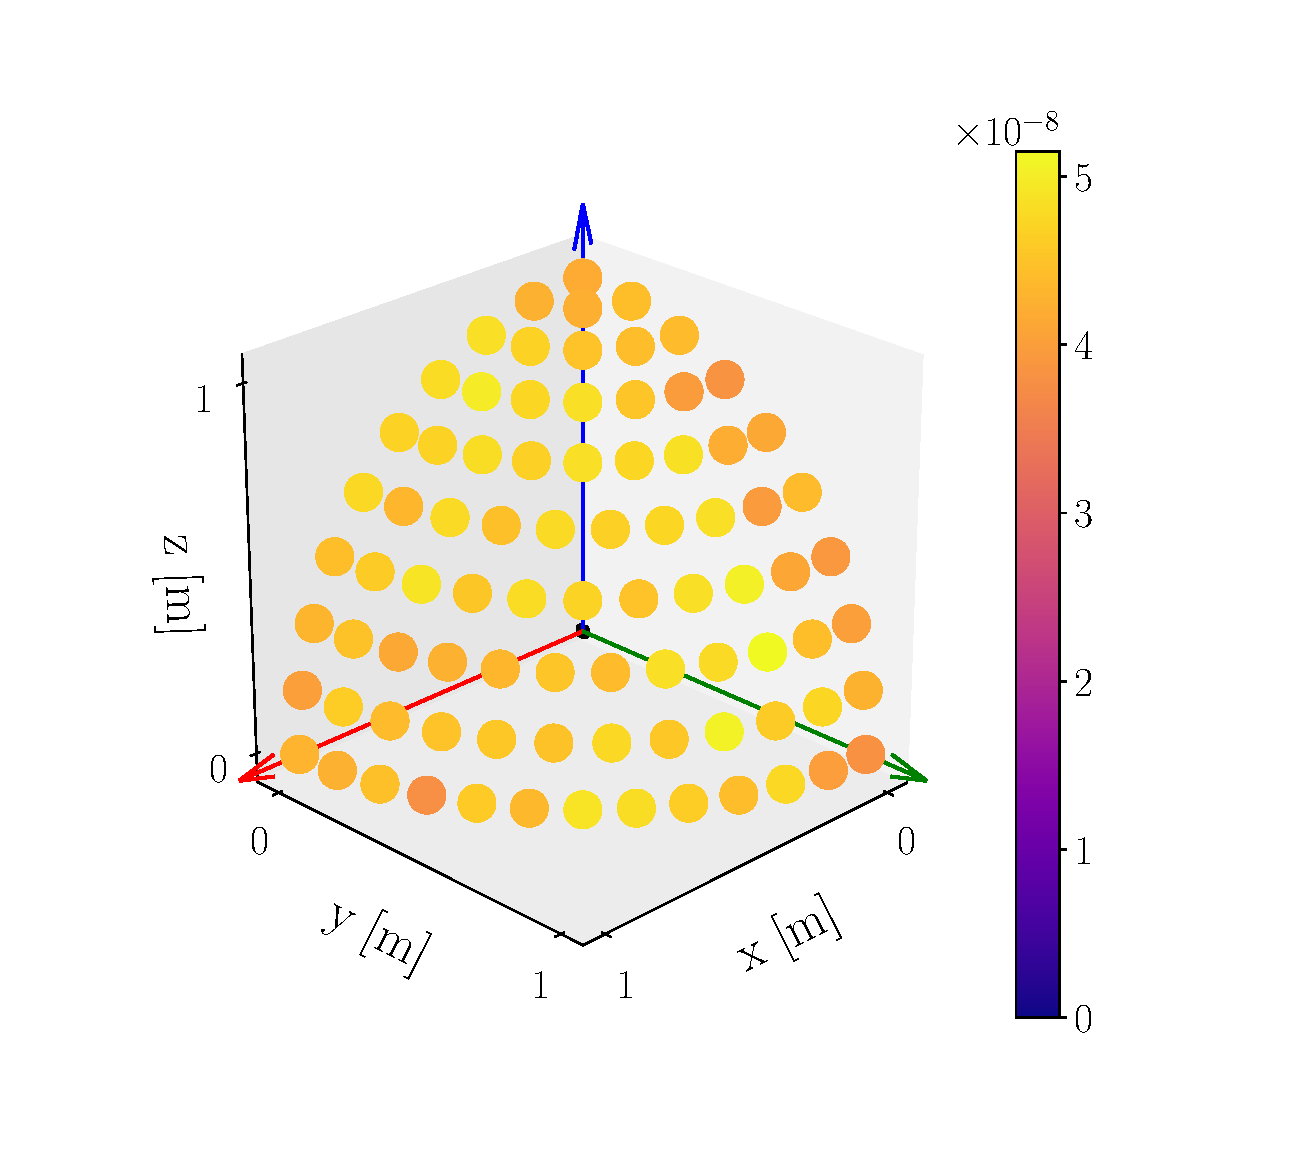
\includegraphics[width=0.42\textwidth,trim={1cm 1cm 2.5cm 1cm},clip]{./fig/photos/monte_carlo_final_prob.eps}
    \label{fig:monte_finalll}
  }
	\centering
  \subfloat[\ac{pix} sensor geometry. The \ac{CdTe} block (grey) has dimensions $14.08 \times 14.08 \times 2 \ \si{\milli\meter}$]{
    \centering
    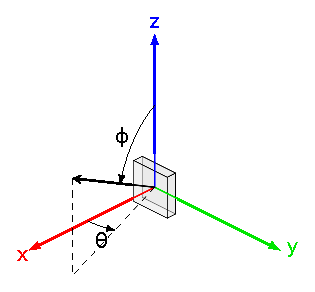
\includegraphics[width=0.4\textwidth]{./fig/photos/axes.eps}
    \label{fig:monte_axes}
  }
  \newline

  \noindent

  \subfloat[$p(\mathrm{reaching\ the\ sensor})$] {
    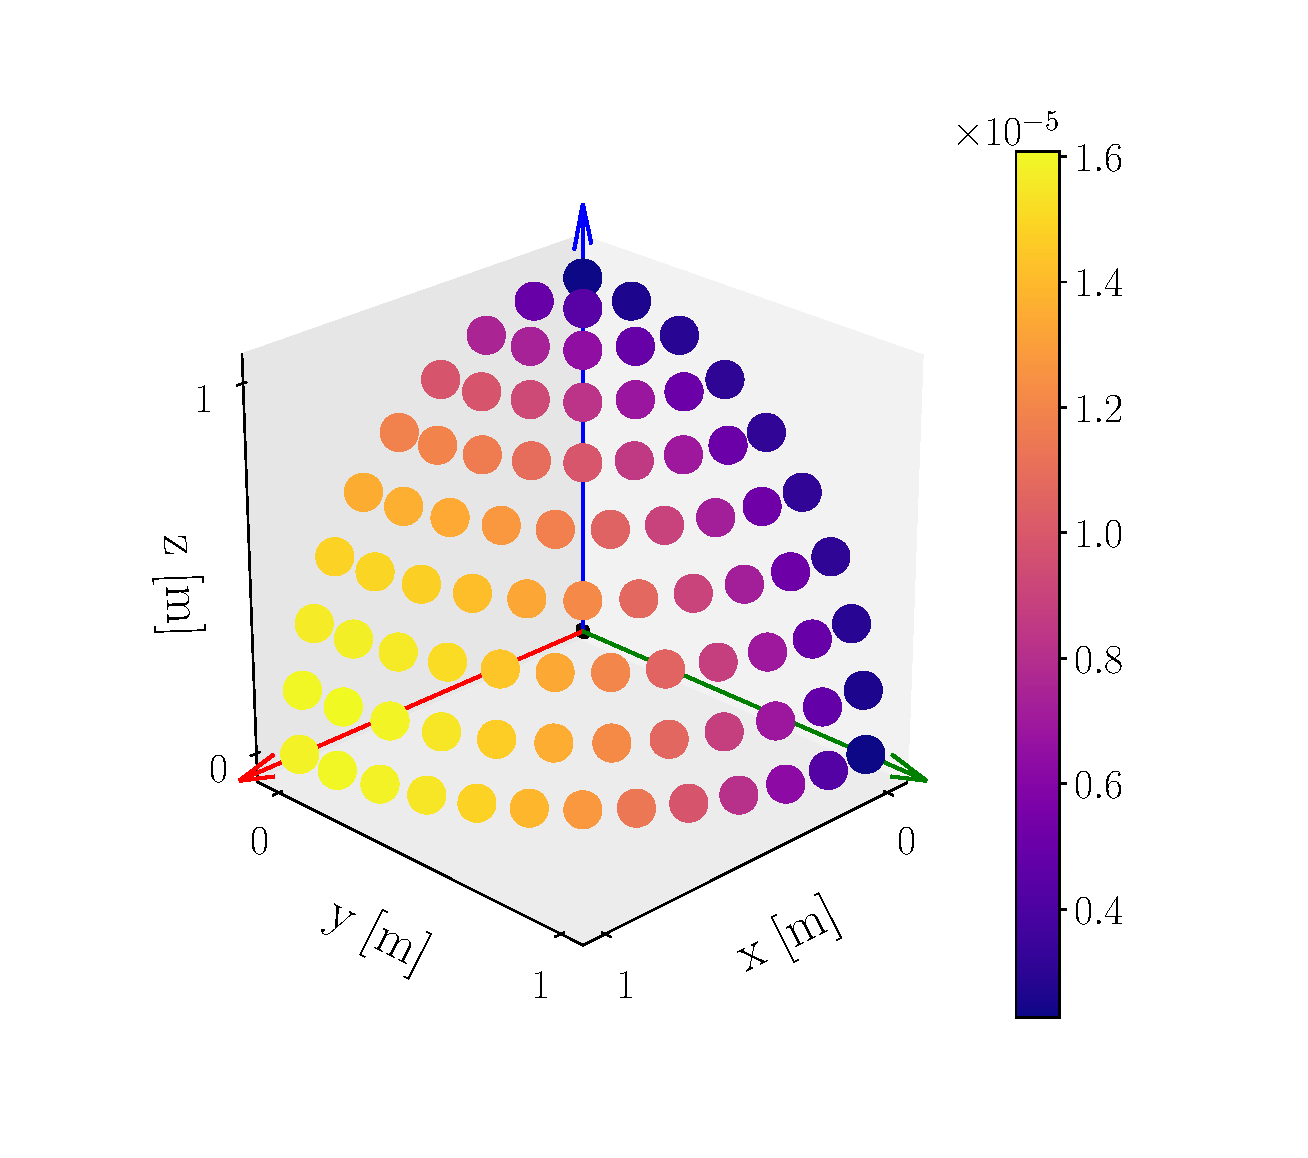
\includegraphics[width=0.42\textwidth,trim={1cm 1cm 1cm 1cm},clip]{./fig/photos/monte_carlo_total_activity.eps}
    \label{fig:monte_reaching}
  }
  \subfloat[$p(\mathrm{cone\ detected}\ |\ \mathrm{reaching\ the\ sensor})$] {
    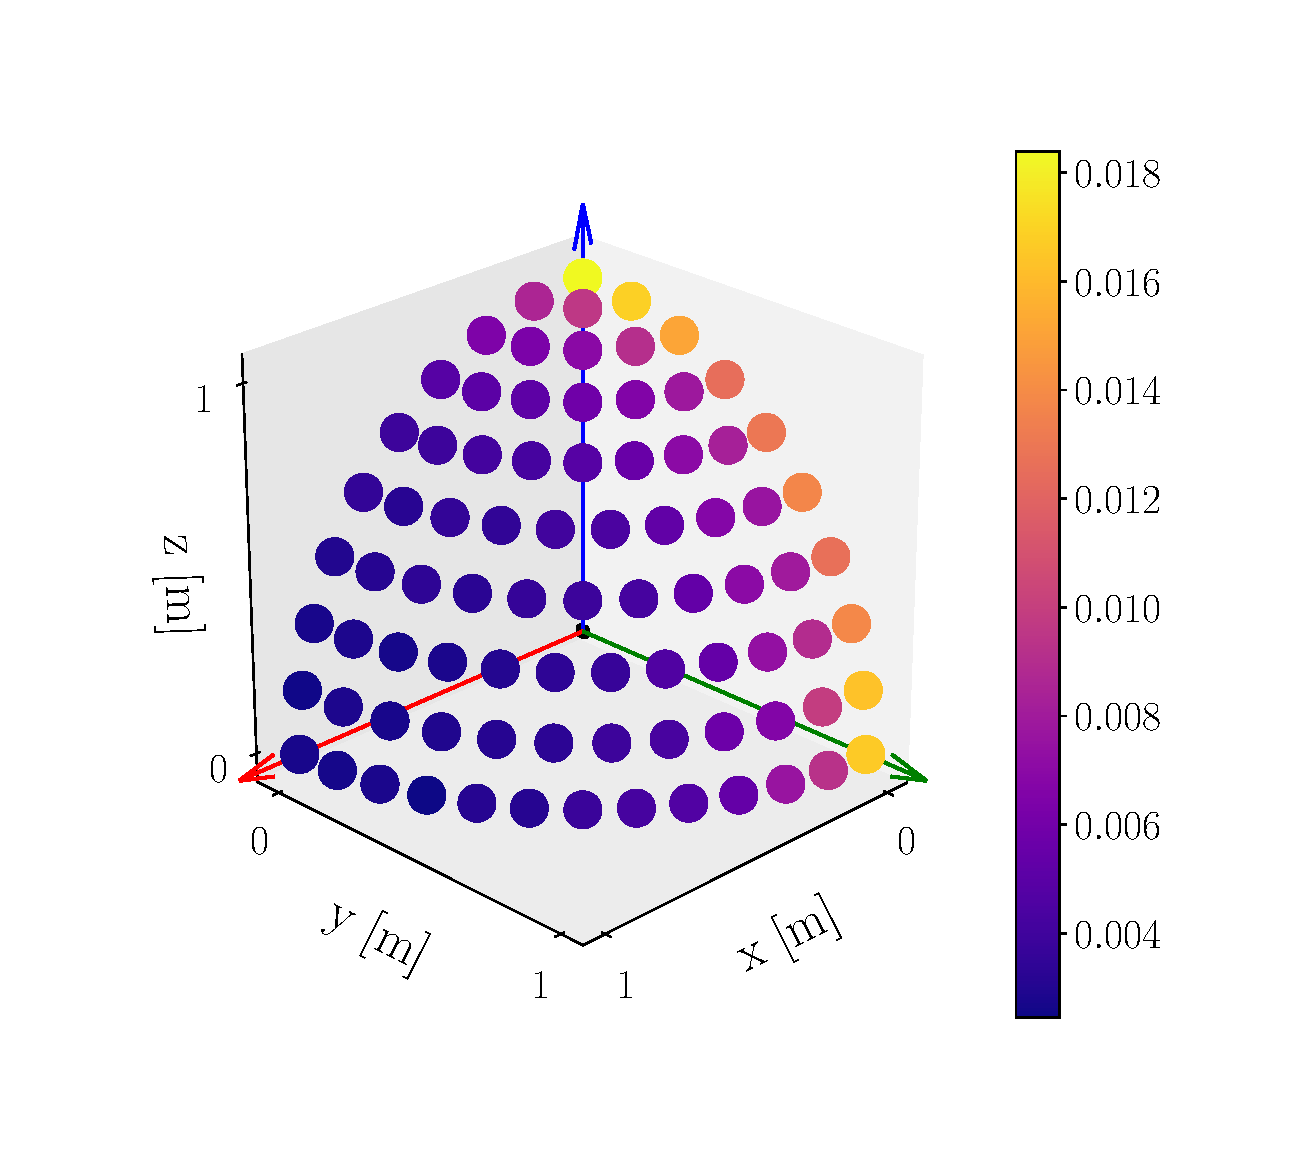
\includegraphics[width=0.42\textwidth,trim={1cm 1cm 1cm 1cm},clip]{./fig/photos/monte_carlo_fraction.eps}
    \label{fig:monte_cone_from_hitting}
  }
  \caption{Direction sensitivity of the \ac{pix} sensor (geometry of the sensor depicted in \protect\subref{fig:monte_axes}). 
  The probability that a $\SI{662}{\kilo\electronvolt}$ photon emitted at the corresponding position causes a Compton cone is depicted in \protect\subref{fig:monte_finalll}. 
  The probability that the particle emitted at a given position reaches the detector is depicted in \protect\subref{fig:monte_reaching}. 
  Lastly, the probability that a photon (that reached the sensor) causes a Compton cone is illustrated in \protect\subref{fig:monte_cone_from_hitting}.}
  \label{fig:monte_clar}
\end{figure}% %%}
%%%%%%%%%%%%%%%%%%%%%%%%%%%%%%%%%%%%%%%%%
\newpage
\section{Evaluation of MLEM method based on real-world data\label{chap:exp1}}
The proposed \ac{MLEM} method for radiation mapping has been tested using data from real-world experiments that were carried out in September 2022 (before the work on this thesis started).
Although the pre-recorded real-world data were collected in realistic conditions with real sensors and sources of ionizing radiation, the prerecorded data do not allow to fully test capabilities of the proposed system.
The reason is the strong dependency between drones trajectories during the experiment and recorded measurements (caused by properties of the ionizing radiation, such as the inverse square law, that is significantly reducing distance from which a radioactive source might be perceived). 
Therefore the outcome of reconstruction strongly depends on in which areas the drones flew during the recorded experiments.

\subsection{Setup and course of the experiment (data collection)}
The area of interest of size $\approx 40 \times 30\ \si{\meter}$ was scanned by a group of four \ac{UAV}s equipped with \ac{pix} sensor.
The \ac{UAV}s were localized using \ac{GPS}.
The drones were controlled by the method proposed in \cite{baca2021gamma}.
In the beginning of the experiment, the drones were following a predefined trajectory covering the whole area of interest uniformly.
After the first 8 Compton cones were detected, three drones were flying $\SI{3}{\meter}$ above the ground encircling the current single-hypothesis estimate of the source position (filtered by a \ac{LKF}). 
The last drone with flight height $\SI{6}{\meter}$ was following a predefined path covering the whole area.
Four sources of Cesium-137 with activity $1900, 500, 180, 50\ \si{\mega\becquerel}$ were located at positions shown in \autoref{e1:gt}.
During the run of the experiment, the drones were mostly encircling the $\SI{500}{\mega\becquerel}$ source position.
The fourth \ac{UAV} flying $\SI{6}{\meter}$ above the ground twice detected photons originating from the $\SI{1900}{\mega\becquerel}$ source. 
As a consequence, the single hypothesis moved towards the strongest source. However, the group of \ac{UAV}s moved back to the $\SI{500}{\mega\becquerel}$ source after a while.
The whole experiment took $\approx \SI{10}{\minute}$, and $263$ Compton cones were recorded.

\subsection{Evaluation of the MLEM method}
The results of the proposed \ac{MLEM} estimation method are presented in \autoref{fig:e1_all}.
The area of interest was discretized with $\SI{1}{\meter}$ resolution, and the number of iterations of the \ac{MLEM} method was set to 10.
The viewpoints (positions of the drones) were sampled with $\SI{5}{\hertz}$, and the \ac{MLEM} estimate was updated every $\SI{2}{\second}$.
The uncertainty of the cone angle  
The final estimate of the emission intensity $\bm{\lambda}$ (based on all data acquired during the experiment) is presented in \autoref{e1:lam}. 
The sensitivity of detection (\autoref{e1:sen}) confirms what was stated before - the drones were mostly encircling the $\SI{500}{\mega\becquerel}$ source at position $(-2, -10)$, which was also correctly localized.
The area in the vicinity of the $\SI{1900}{\mega\becquerel}$ source at position $(16, 0)$ was much less explored by the \ac{UAV}s (and therefore fewer Compton cones originating there were recorded).
Despite the much lower sensitivity in that area, the \ac{MLEM} method estimated some local maxima in the neighbourhood of the true position of the strongest source.
The two weakest sources of radiation are indistinguishable from the noise.



\mycomment{% %%{
  \subsection{Convergence of the MLEM algorithm}
The convergence of \ac{MLEM} algorithm (using \ac{MSE} as the metric) is shown in \autoref{e1:mse}. 
\ac{MSE} in this scenario is defined as
\begin{equation}
MSE = \frac{1}{J} \sum_{j = 0}^{J} (\lambda_{j_{normalized}} - g_{j})^{2},
\end{equation}
where the ground truth is defined as $g_{j} = \frac{\mathrm{source\ activity}}{\mathrm{max}(\mathrm{source\ activity})}$ at the sources locations and $g_{j} = 0$ elsewhere.
The iterative \ac{MLEM} algorithm is initialized with back-projection (\autoref{e1:bp}). 
We can see in \autoref{e1:mse} that the decrease of the $MSE$ stopped after a few iterations.

\begin{figure}
	\centering
    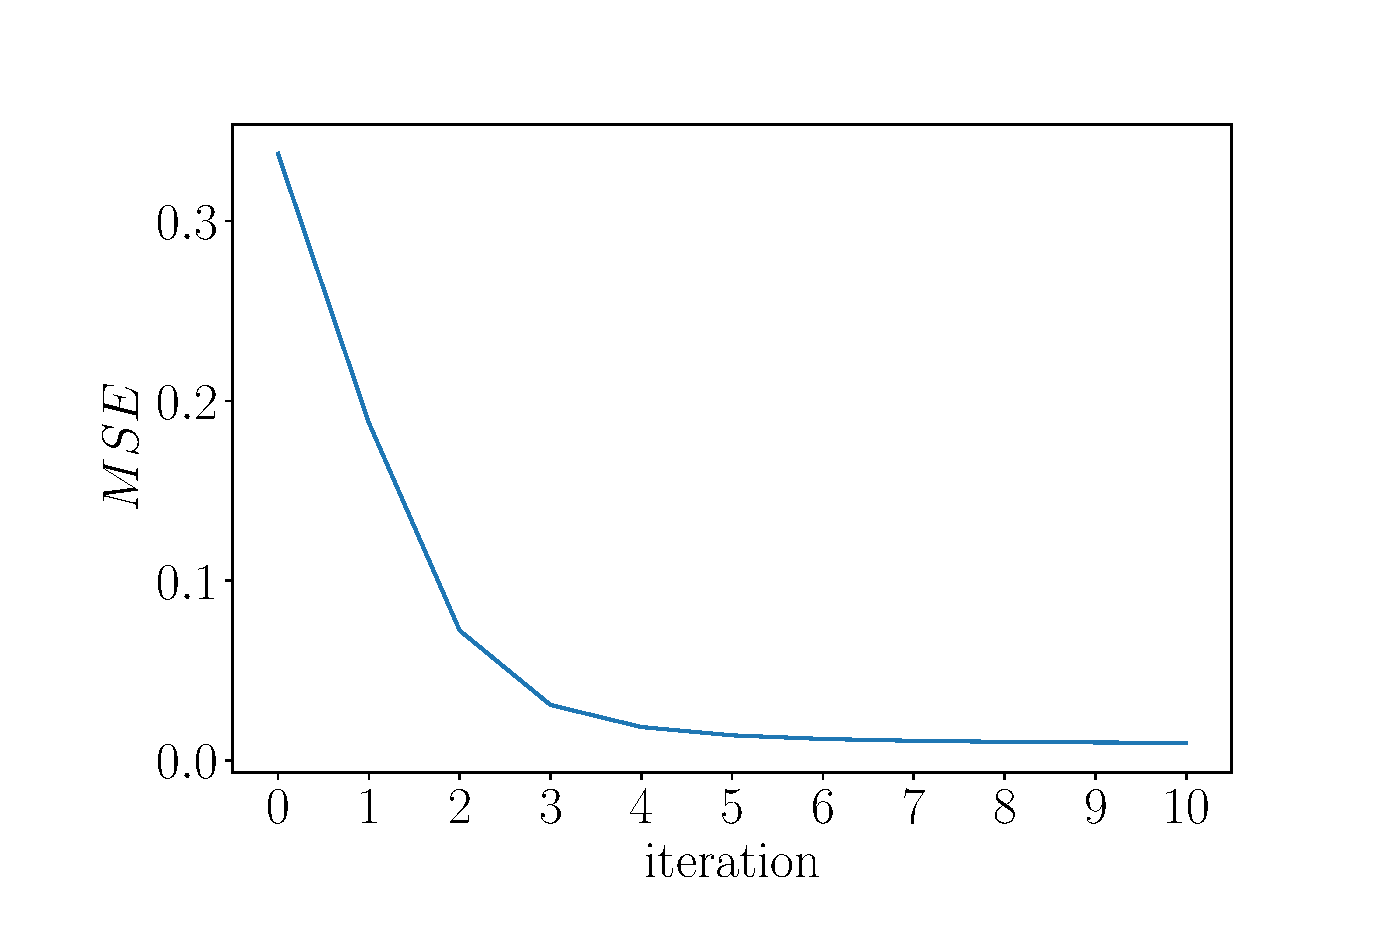
\includegraphics[width=0.5\textwidth,trim={0 0.5cm 2cm 1cm},clip]{./fig/photos/auto_mse_realworld.eps}
		\caption{\ac{MSE} of the \ac{MLEM} method applied to the pre-recorded data from real-world experiments.}
    \label{e1:mse}
\end{figure}
}% %%}



\begin{figure}[!htb]% %%{
  \centering
  \subfloat[estimate of ionizing radiation intensity $\bm{\lambda}$ (rescaled)] {
    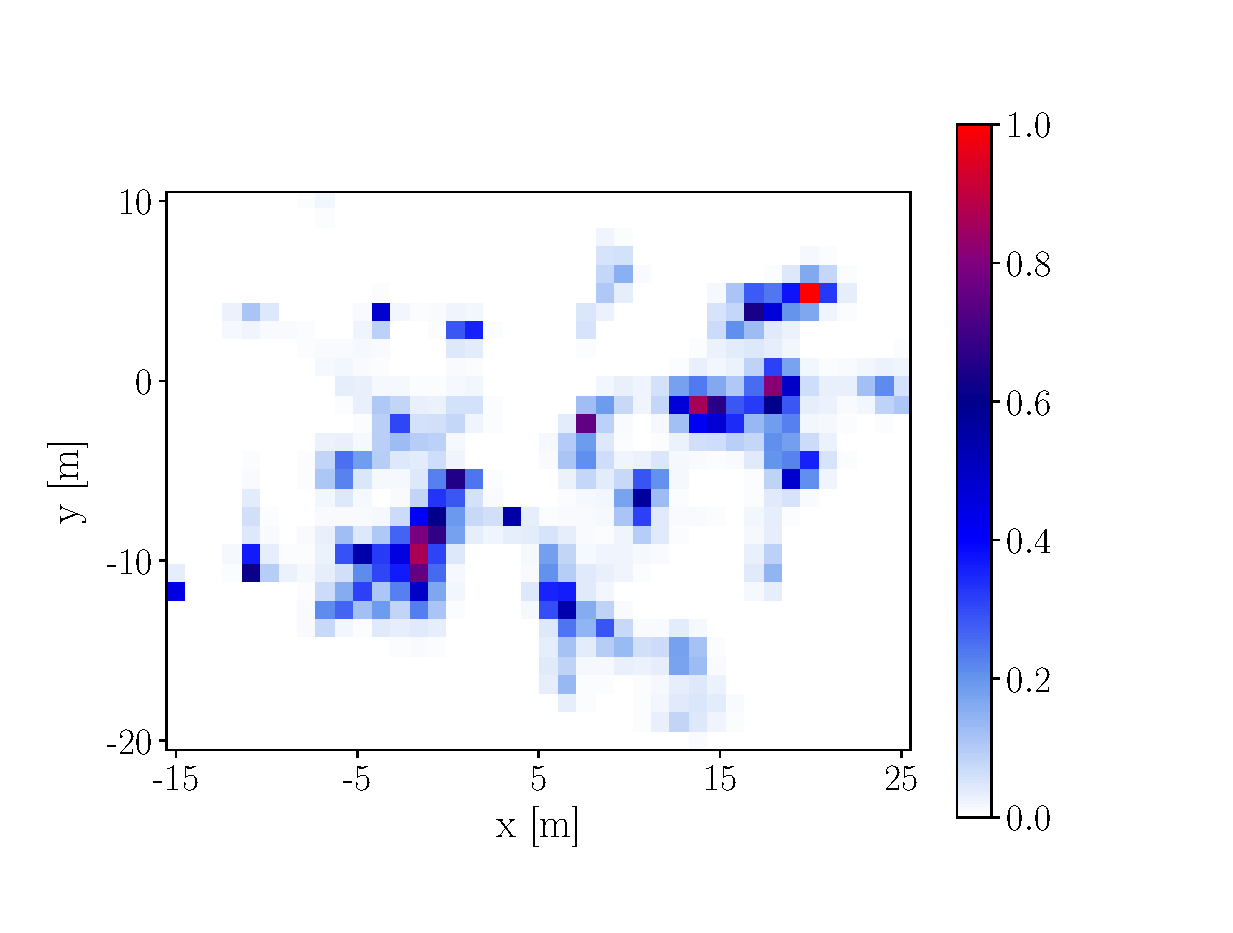
\includegraphics[width=0.5\textwidth,trim={0 0.5cm 2cm 1cm},clip]{./fig/photos/auto_lam.eps}
    \label{e1:lam}
  }
  \subfloat[ground truth positions of sources ($\si{\mega\becquerel}$)] {
    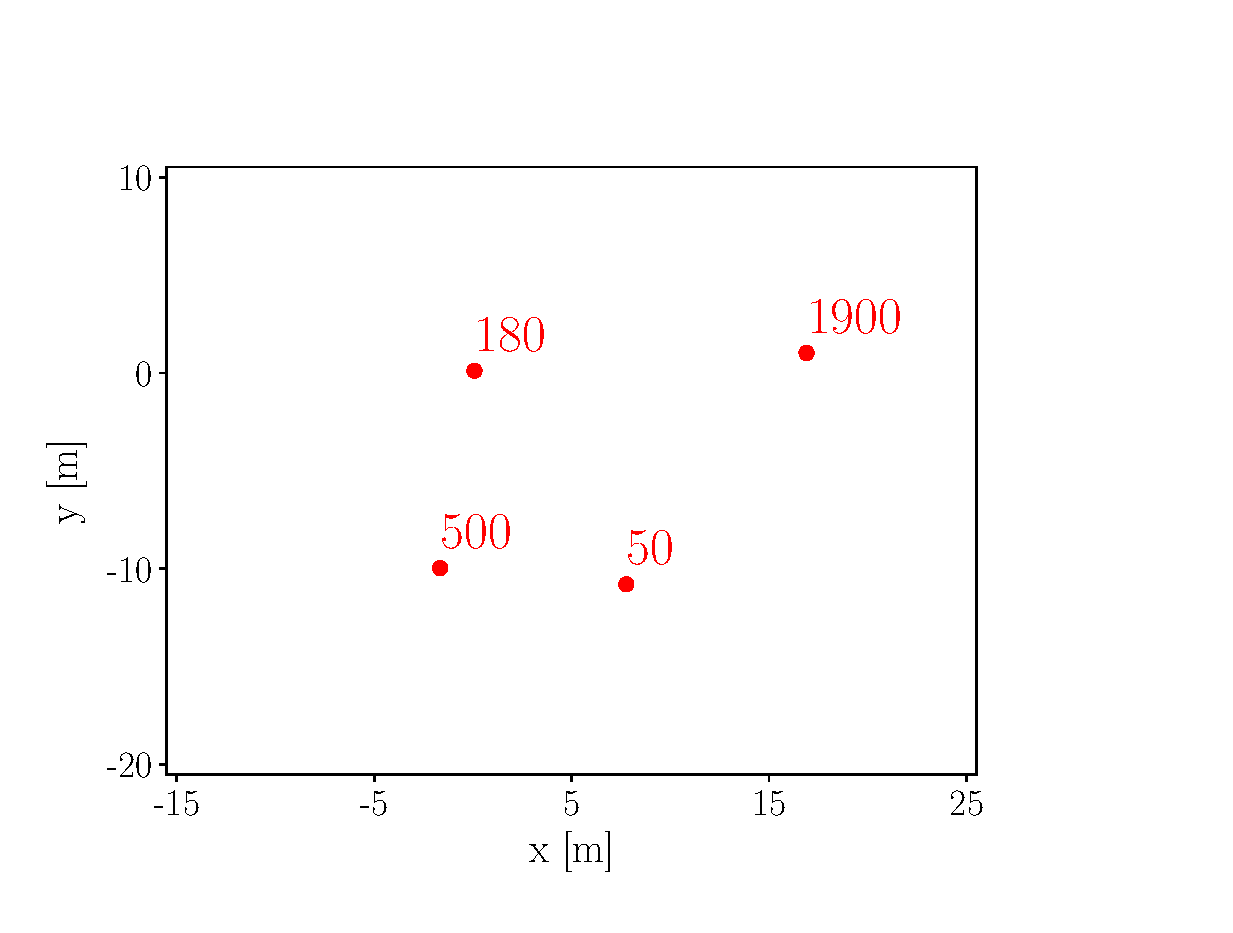
\includegraphics[width=0.5\textwidth,trim={0 0.5cm 2cm 1cm},clip]{./fig/photos/auto_gt.eps}
    \label{e1:gt}
  }
  \newline
  \noindent 
  \subfloat[back-projection (number of Compton cones)] {
    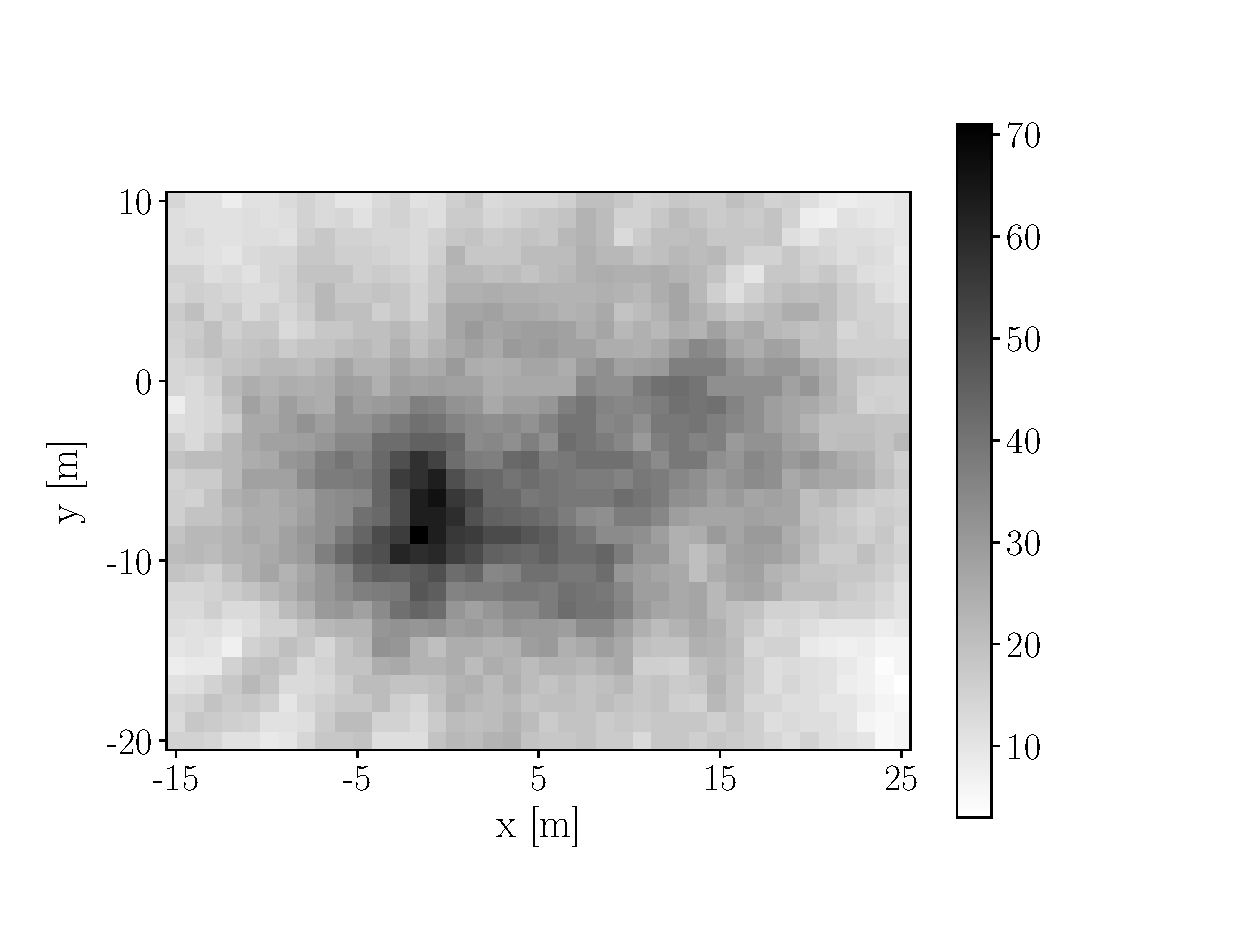
\includegraphics[width=0.5\textwidth,trim={0 0.5cm 2cm 1cm},clip]{./fig/photos/auto_bp.eps}
    \label{e1:bp}
  }
  \subfloat[sensitivity of detection $\mathbf{s}$] {
    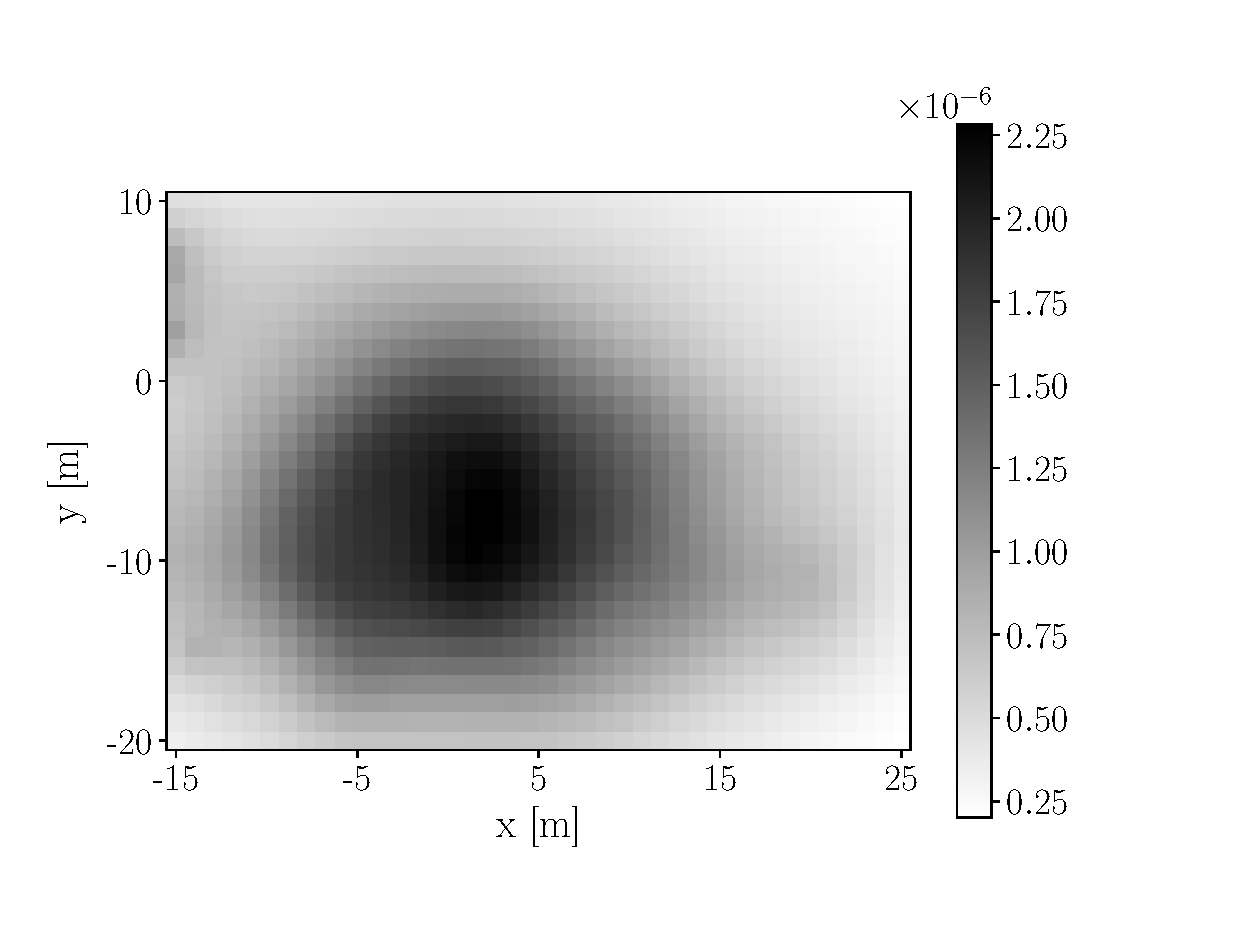
\includegraphics[width=0.5\textwidth,trim={0 0.5cm 2cm 1cm},clip]{./fig/photos/auto_sen.eps}
    \label{e1:sen}
  }
  \caption{The \ac{MLEM} method evaluated on pre-recorded real-world data.}
  \label{fig:e1_all}
\end{figure}% %%}
%%%%%%%%%%%%%%%%%%%%%%%%%%%
\subsection{Summary}
The results of the \ac{MLEM} reconstruction are heavily affected by a noise in measurements.
First of all, the \ac{UAV}s were localized using \ac{GPS} method that might be effected by a position error of several meters.
The position error propagates to the uncertainty of the Compton cone origins.
Furthermore, the real \ac{pix} sensors produced many outliers --- e.g. Compton cones pointing upwards or not intersecting any source position. 
The noisy measurements are probably caused by the working principle of an unshielded single-layer Compton camera, where ionizing particles coming from different directions might affect the Cone reconstruction procedure.
This might be a limiting factor for the localization of multiple sources of ionizing radiation (with high emission activity) that are close to each other.
The single-layer Compton camera is able to estimate the direction of incoming ionizing photons only if the number of interactions detected by the Timepix3 pixel detector inside the \ac{pix} sensor is relatively low and corresponding interactions can be paired together correctly.
However, the presence of multiple sources in close vicinity increases the particle flux and may potentially increase the number of outliers.

In summary, the comparison of \ac{MLEM} estimate (\autoref{e1:lam}) and back-projection (\autoref{e1:bp}) show that the \ac{MLEM} significantly improved the reconstruction quality.
The $\SI{1900}{\mega\becquerel}$ source was localized (despite the low number of recorded photons originating there) 
thanks to the weighting of the estimate with the sensitivity of detection in the \ac{MLEM} algorithm.
Better results might be achieved by using an active search strategy, where the drones are controlled in order to improve the quality of the current \ac{MLEM} estimate.









%%%%%%%%%%%%%%%%%%%%%%%%%%%%%%%%%%%%%%%%%%%%%%%%%%%%%%%%
%%%%%%%%%%%%%%%%%%%%%%%%%%%%%%%%%%%%%%%%%%%%%%%%%%%%%%%%%%%%%%%%%%%%%
%%%%%%%%%%%%%%%%%%%%%%%%%%%%%%%%%%%%%%%%%%%%%%%%%%%%%%%%%%%%%%

\section{Evaluation of MLEM and search strategy in simulation\label{chap:exp2}}
The \ac{MLEM} estimation method has been tested together with the proposed search strategy in \textit{Gazebo} simulator. 
The results were compared with the back-projection method, that served as a baseline.

\begin{figure}[!htb]
  \centering
    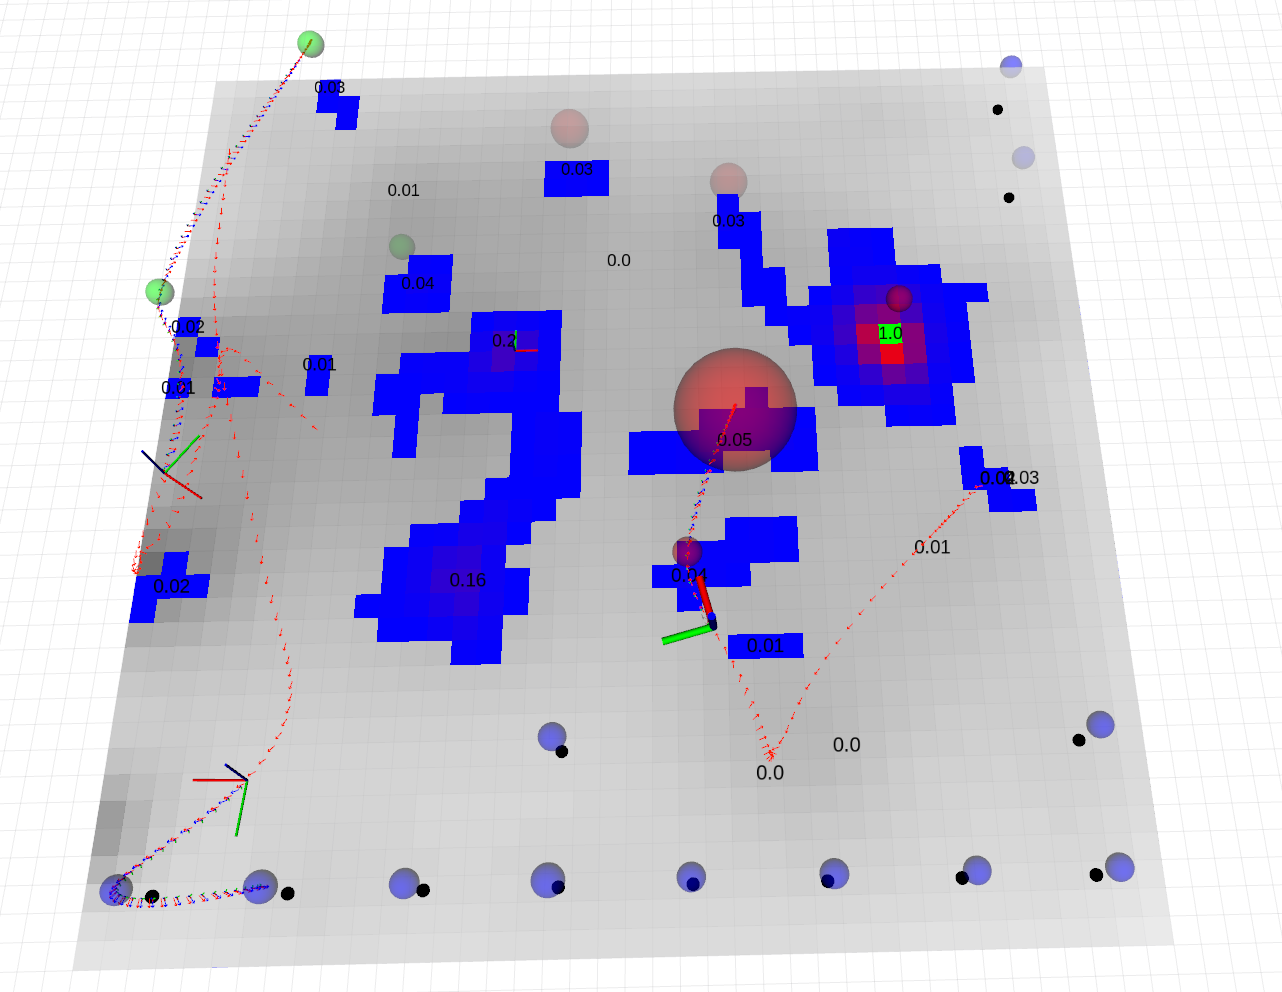
\includegraphics[width=0.9\textwidth]{./fig/photos/simu_search.png}
  \caption{Experiments in \textit{Gazebo} simulator. The \ac{UAV}s are autonomously mapping sources of ionizing radiation place in the area $40 \times 40\ \si{\meter}$ (resolution $r = \SI{1}{\meter}$). 
  The current \ac{MLEM} estimate is visualized using blue-red-green distribution and black numbers denoting the relative activity of local maxima at the given position. 
  The drones follow the trajectories (red arrows) to visit waypoints (depicted as transparent spheres). Two drones are designated for exploitation (red and green waypoints) and one for exploration (blue waypoints).}
  \label{fig:simu_search}
\end{figure}

\subsection{Experiment setup}
The distribution and activity of the radioactive sources were the same as in the real-world experiments described in the previous section.
Three drones flying $\SI{3}{\meter}$ above the ground were used during the experiment.  
The simulation process (visualized in \textit{RViz}) is shown in \autoref{fig:simu_search}.
Two drones were designated for exploitation (visiting the positions where the sources of radiation are present based on the latest \ac{MLEM} estimate), and one for exploration (visiting positions with the lowest sensitivity). 
The drones were initialized at positions ($-15, -10$), ($-5, -10$) and ($5, -10$) and controlled by the proposed search strategy in the rest of the experiment.
\subsubsection{Measurement noise}
Extra noise was added to the measurements to model the real-world conditions.
The inaccuracy in the drone position (resulting in the shifted origin of the Compton cone) was modelled with the Normal distribution $\mathcal{N}(\mu_{pos}, \sigma_{pos})$ with zero means $\mu_{pos} = 0$ and standard deviation $\sigma_{pos} = \SI{1.5}{\meter}$. 
The noise in energy measurements of the simulated \ac{pix} sensor was modeled the Normal distribution $\mathcal{N}(\mu_{energy}, \sigma_{energy})$ with zero mean $\mu_{energy} = 0$ and standard deviation $\sigma_{energy} = \SI{7}{\kilo\electronvolt}$.

\subsection{Results}
The results of the \ac{MLEM} reconstruction are presented in \autoref{fig:e2}.
The progress of radiation mapping is illustrated in \autoref{e2:lam1} (time $t = \SI{25}{\second}$) and \autoref{e2:lam2} ($t = \SI{100}{\second}$), corresponding sensitivity of detection is presented in \autoref{e2:sen1}, \autoref{e2:sen2}.
The active search strategy controlled the drones in order to acquire more measurements, which significantly improved the initial inaccurate estimate (based on a smaller number of Compton cones).
We may notice that after $\SI{100}{\second}$ of flight the \ac{UAV}s correctly localized the $\SI{1900}{\mega\becquerel}$ , $\SI{500}{\mega\becquerel}$ and $\SI{280}{\mega\becquerel}$ sources of simulated ionizing radiation.
The $\SI{50}{\mega\becquerel}$ source was not recognized due to its low emission activity or because it was filtered out during the later iterations of the \ac{MLEM} algorithm.
The \ac{MLEM} method significantly improved the solution compared to the back-projection illustrated in \autoref{e2:bp}.

\subsection{Summary}
Three sources with the highest emission activity were correctly localized in less than $\SI{100}{\second}$.
The proposed \ac{MLEM} estimation method, together with the autonomous search strategy, worked as intended.
Although the \ac{MLEM} method does not estimate the positions of sources perfectly for a small number of measurements, the active search strategy guides the \ac{UAV}s in order to acquire more measurements, which further improves the estimate's quality.
The extensive testing in simulations showed that the inaccuracy in the Compton cones' origins significantly reduces the quality of reconstruction, which highlights the need for accurate localization of drones during real-world experiments.
In summary, the experiment showed that the proposed method is capable of autonomous localization of multiple sources of ionizing radiation (of different emission activity).




\subsubsection{Simulation vs. reality}
The simulated noise in the drone's position and energies helped to bring the simulation closer to real-world conditions.
However, the used simulator of ionizing radiation simulates each source-sensor pair independently, which ignores the fact that ionizing particles from multiple sources might interact in the sensor at the same time (causing outliers), therefore the simulation is not as accurate as it could be.
Improving the simulator in order to process interactions caused by different sources simultaneously presents a possible direction for future research.

\begin{figure}[!htb]% %%{
  \centering
  \subfloat[($t = \SI{25}{\second}$) source intensities $\bm{\lambda}$ (rescaled) ] {
    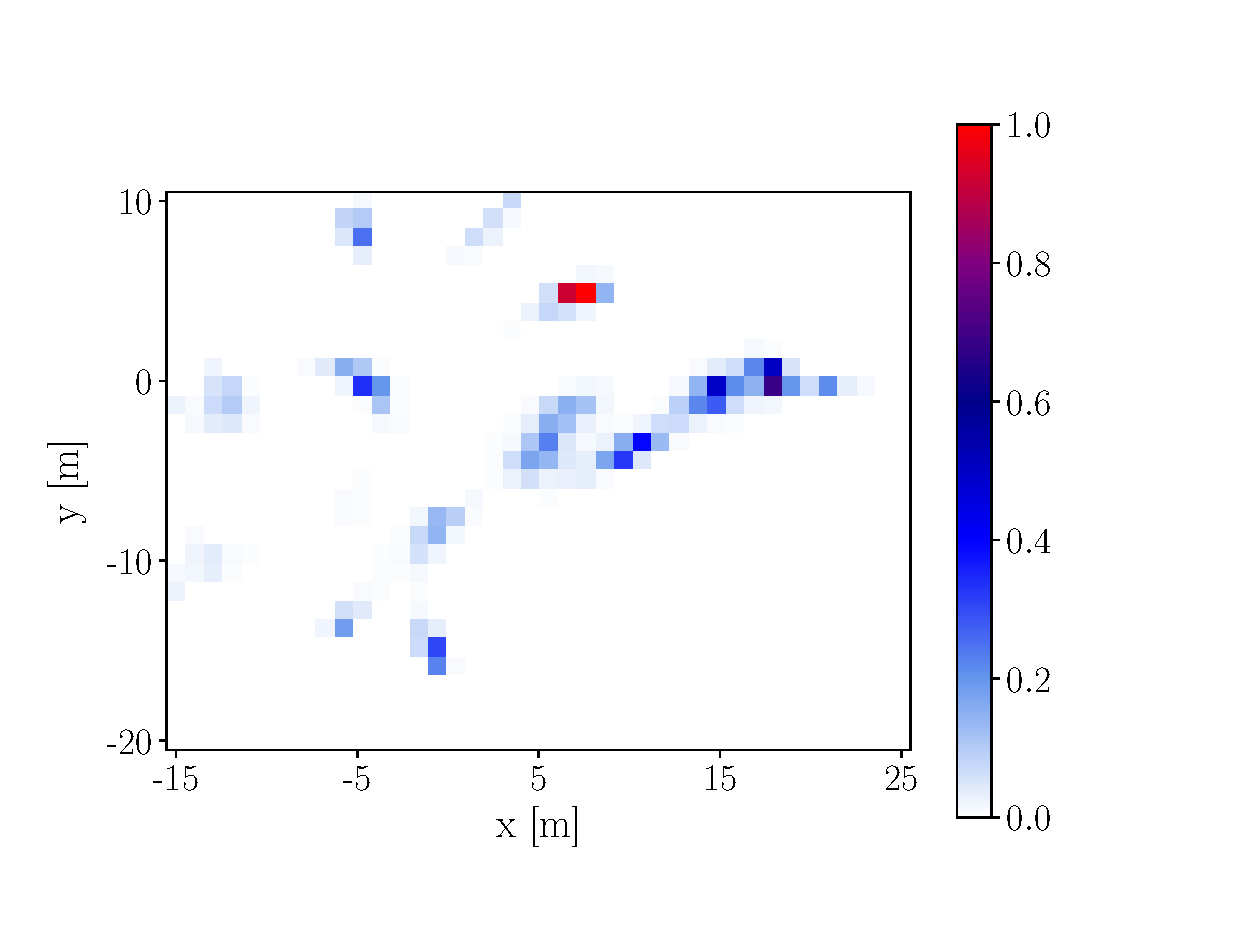
\includegraphics[width=0.5\textwidth,trim={0 0.5cm 2cm 1cm},clip]{./fig/photos/auto_simulation_lam_1.eps}
    \label{e2:lam1}
  }
  \subfloat[($t = \SI{25}{\second}$) sensitivity of detection $\mathbf{s}$ ] {
    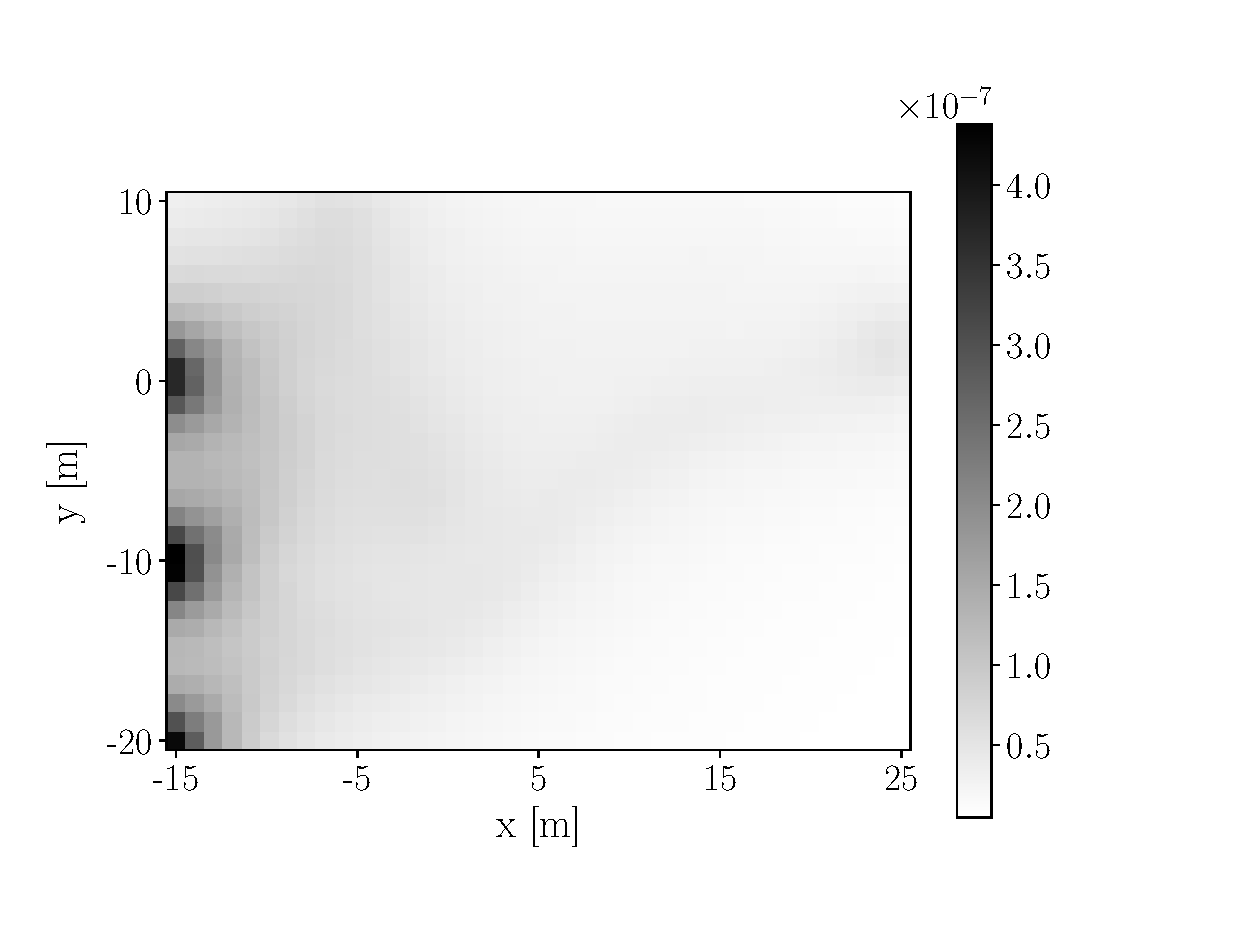
\includegraphics[width=0.5\textwidth,trim={0 0.5cm 2cm 1cm},clip]{./fig/photos/auto_simulation_sen_1.eps}
    \label{e2:sen1}
  }
  \newline
  \noindent
  \subfloat[($t = \SI{100}{\second}$) source intensities $\bm{\lambda}$ (rescaled) ] {
    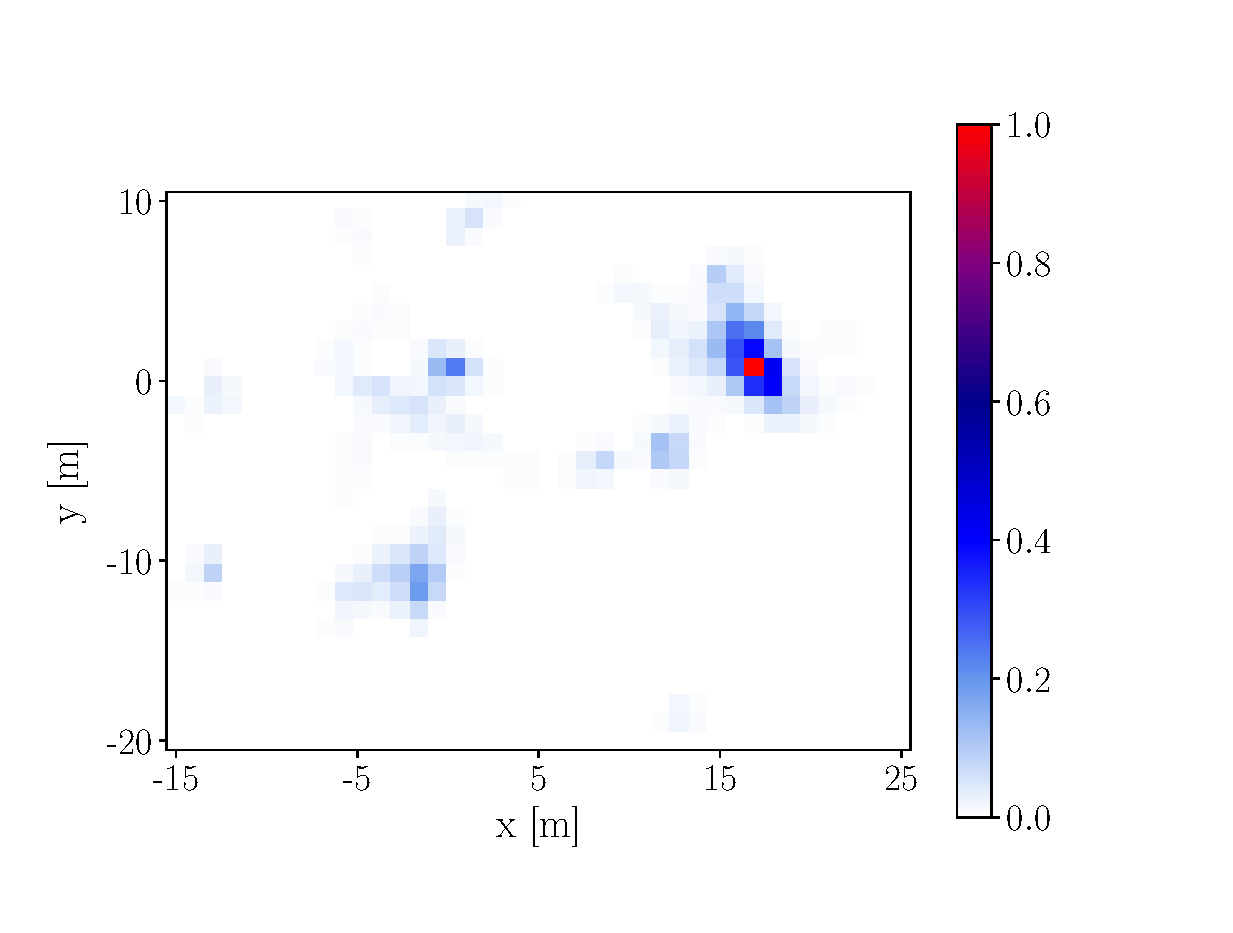
\includegraphics[width=0.5\textwidth,trim={0 0.5cm 2cm 1cm},clip]{./fig/photos/auto_simulation_lam_2.eps}
    \label{e2:lam2}
  }
  \subfloat[($t = \SI{100}{\second}$) sensitivity of detection $\mathbf{s}$ ] {
    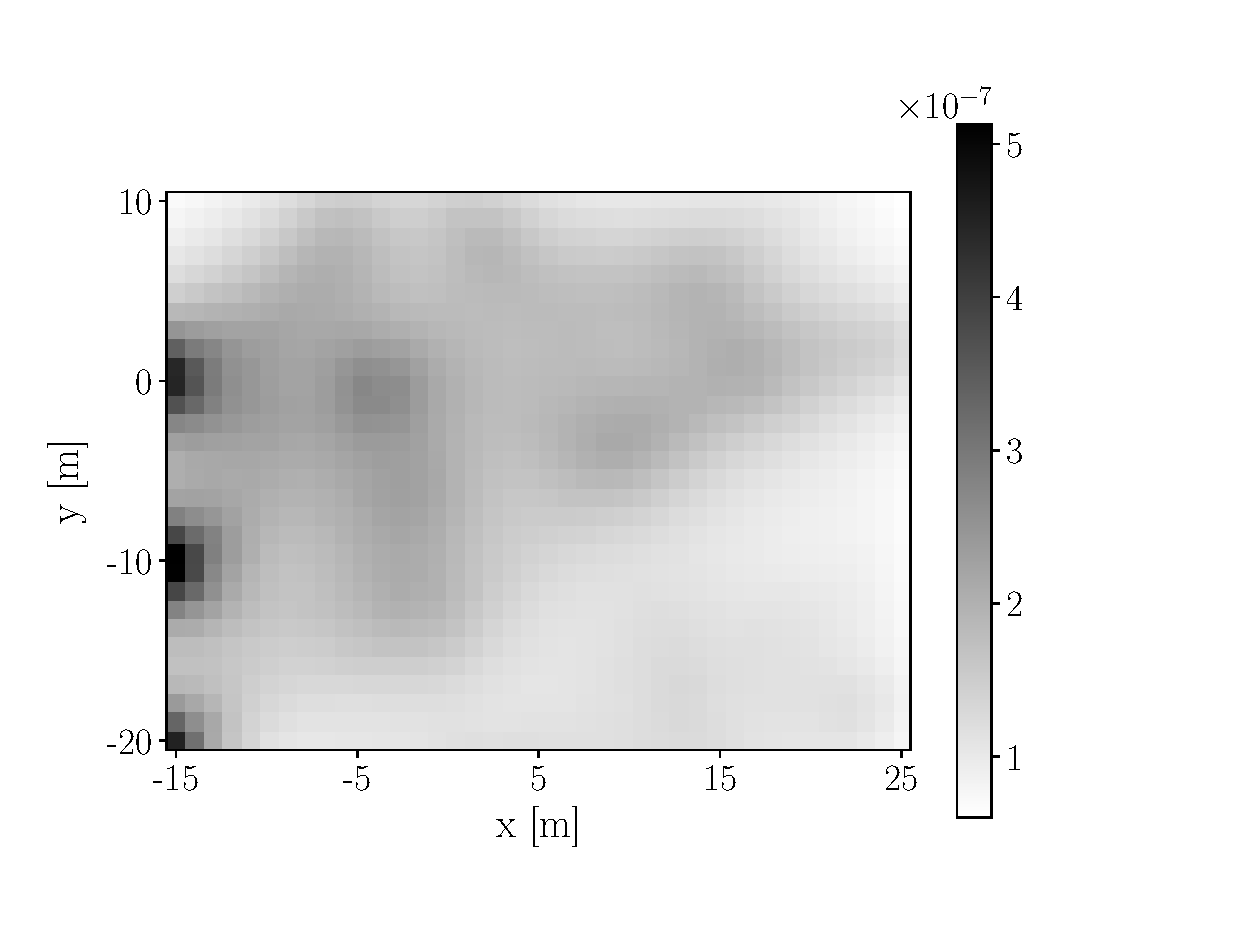
\includegraphics[width=0.5\textwidth,trim={0 0.5cm 2cm 1cm},clip]{./fig/photos/auto_simulation_sen_2.eps}
    \label{e2:sen2}
  }
  \newline
  \noindent
  \subfloat[($t = \SI{100}{\second}$) back projection (number of cones)] {
    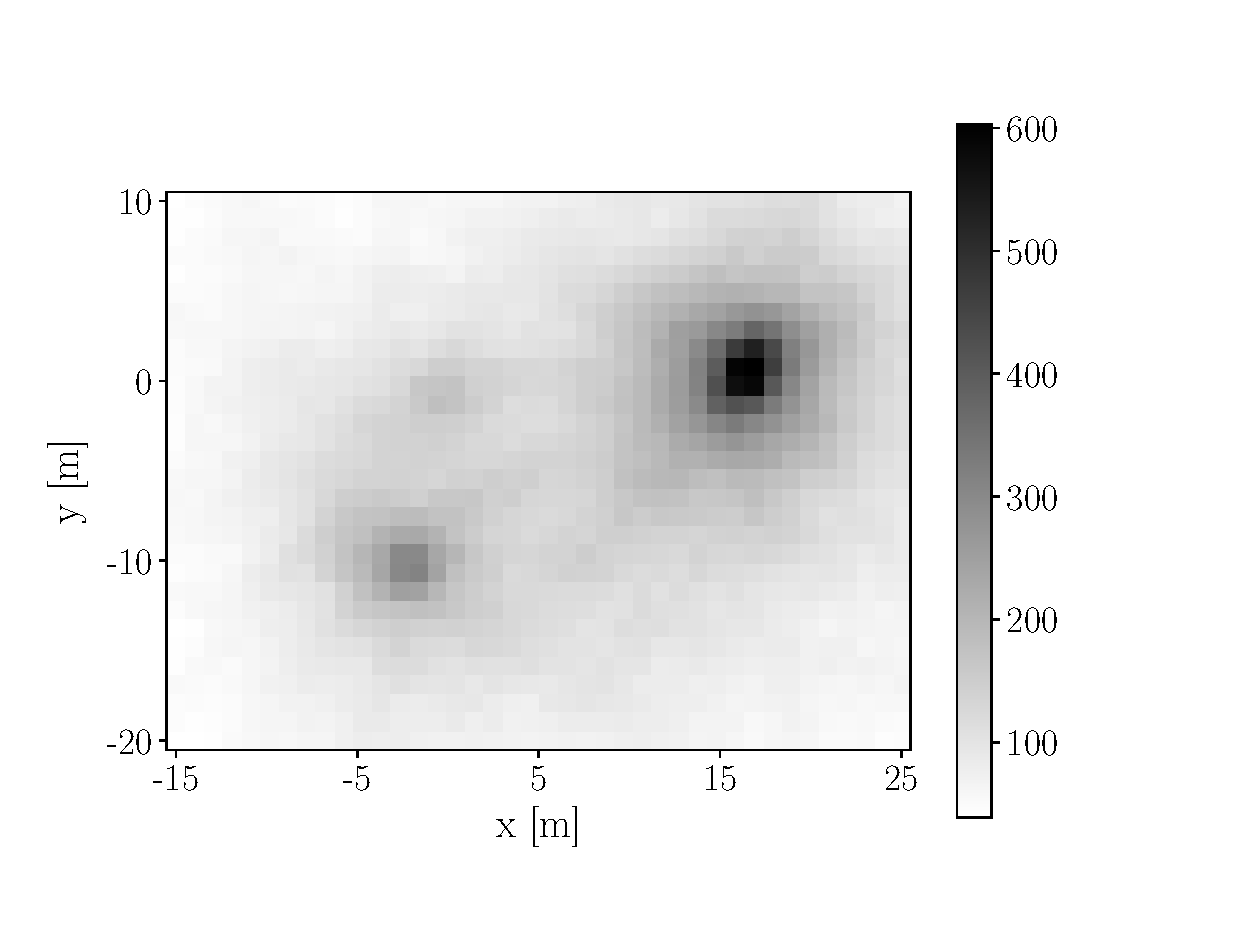
\includegraphics[width=0.5\textwidth,trim={0 0.5cm 2cm 1cm},clip]{./fig/photos/auto_simulation_bp.eps}
    \label{e2:bp}
  }
  \subfloat[ground truth positions of sources ($\si{\mega\becquerel}$)] {
    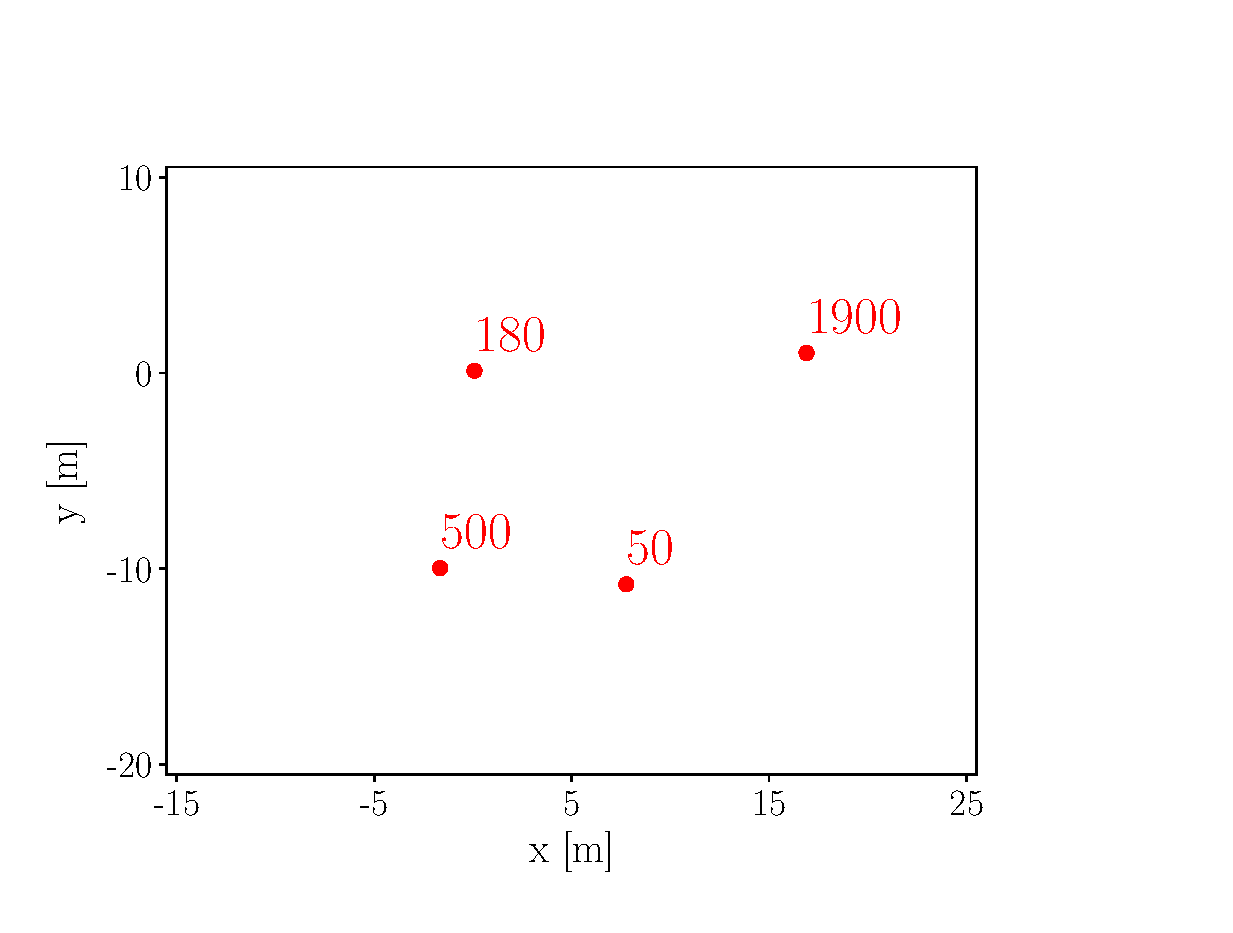
\includegraphics[width=0.5\textwidth,trim={0 0.5cm 2cm 1cm},clip]{./fig/photos/auto_simulation_gt.eps}
    \label{e2:gt}
  }
  \caption{Results of the experiment with three \ac{UAV}s and four sources of ionizing radiation simulated in \textit{Gazebo}. 
  The progress of the \ac{MLEM} reconstruction method is shown in \protect\subref{e2:lam1}, \protect\subref{e2:sen1} and \protect\subref{e2:lam2}, \protect\subref{e2:sen2}.
  %The output of the \ac{MLEM} method after $\SI{25}{\second}$ (\autoref{e2:lam1}, \autoref{e1:sen1}) and after $\SI{100}{\second}$ (\autoref{e2:lam2}, \autoref{e1:sen2}) is presented. 
  %We can see that the quality of the \ac{MLEM} estimate improved during the flight thanks to the active search strategy.
  The back-projection of all cones measured in the first $\SI{100}{\second}$ is shown in \protect\subref{e2:bp}.  }
  \label{fig:e2}
\end{figure}% %%}


\mycomment{
\begin{figure}[!htb]% %%{
  \centering
  \subfloat[($t = \SI{25}{\second}$) source intensities $\bm{\lambda}$ (rescaled) ] {
    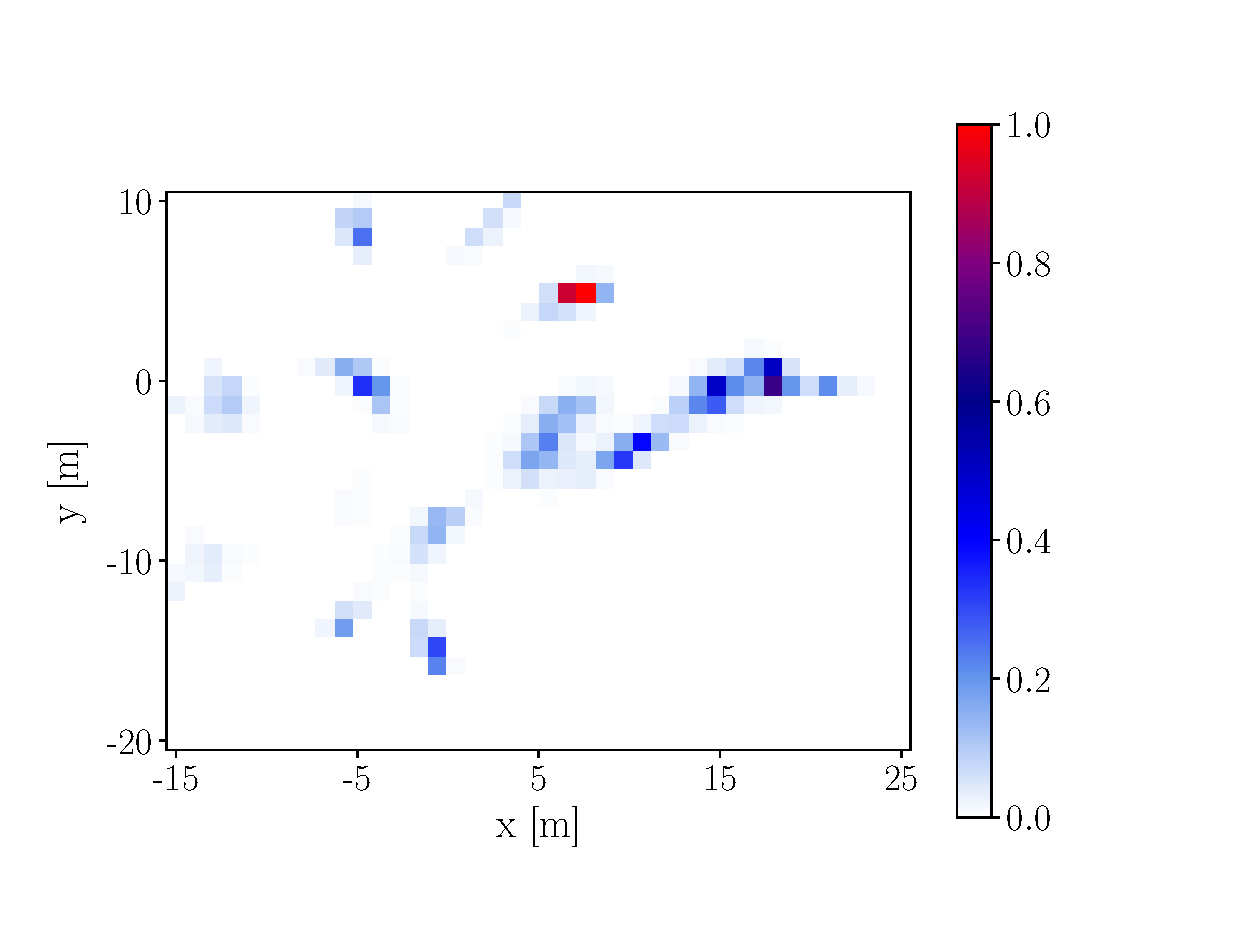
\includegraphics[width=0.5\textwidth,trim={0 0.5cm 2cm 1cm},clip]{./fig/photos/auto_simulation_lam_1.eps}
    \label{e2:lam1}
  }
  \subfloat[($t = \SI{25}{\second}$) sensitivity of detection $\mathbf{s}$ ] {
    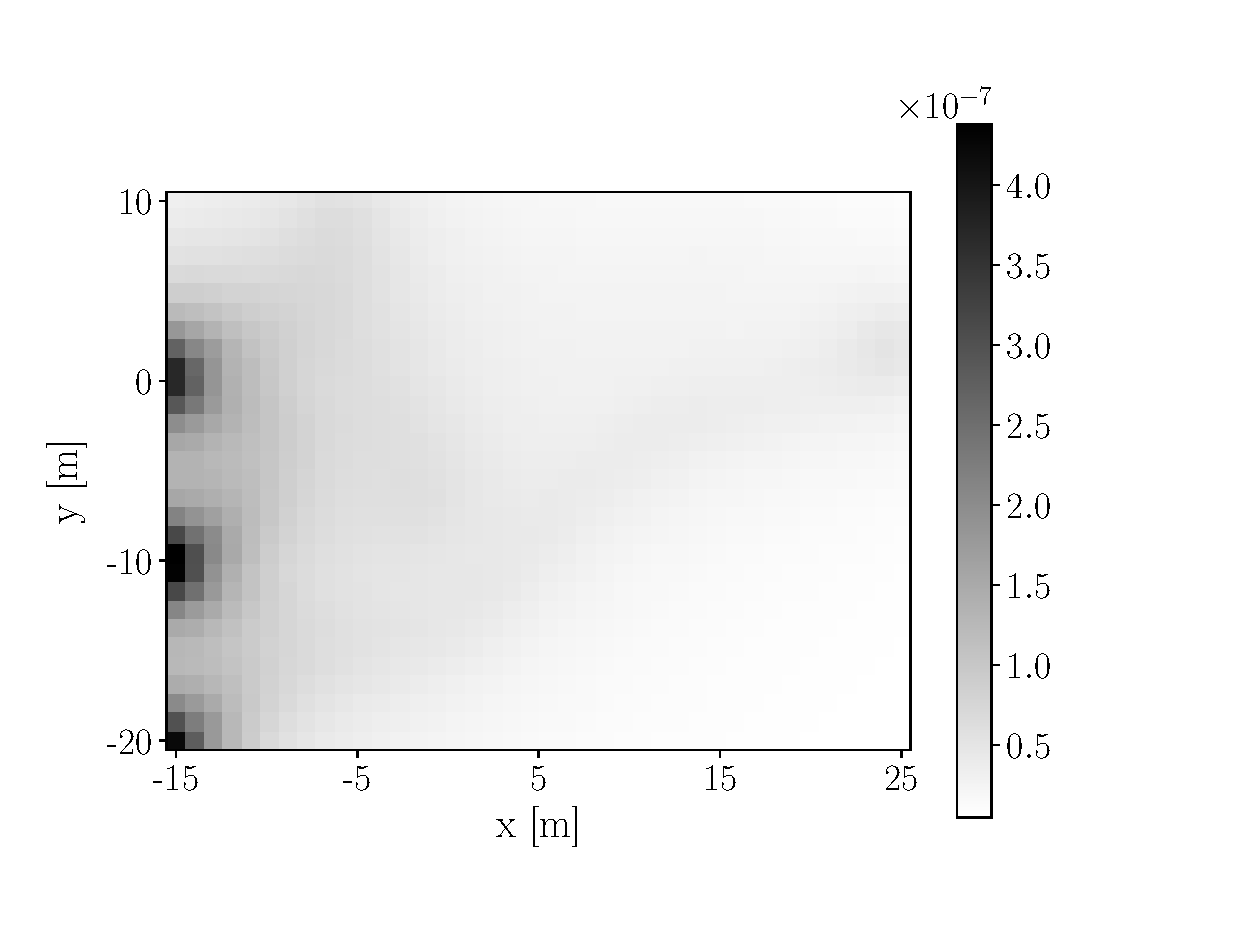
\includegraphics[width=0.5\textwidth,trim={0 0.5cm 2cm 1cm},clip]{./fig/photos/auto_simulation_sen_1.eps}
    \label{e2:sen1}
  }
  \newline
  \noindent
  \subfloat[($t = \SI{100}{\second}$) source intensities $\bm{\lambda}$ (rescaled) ] {
    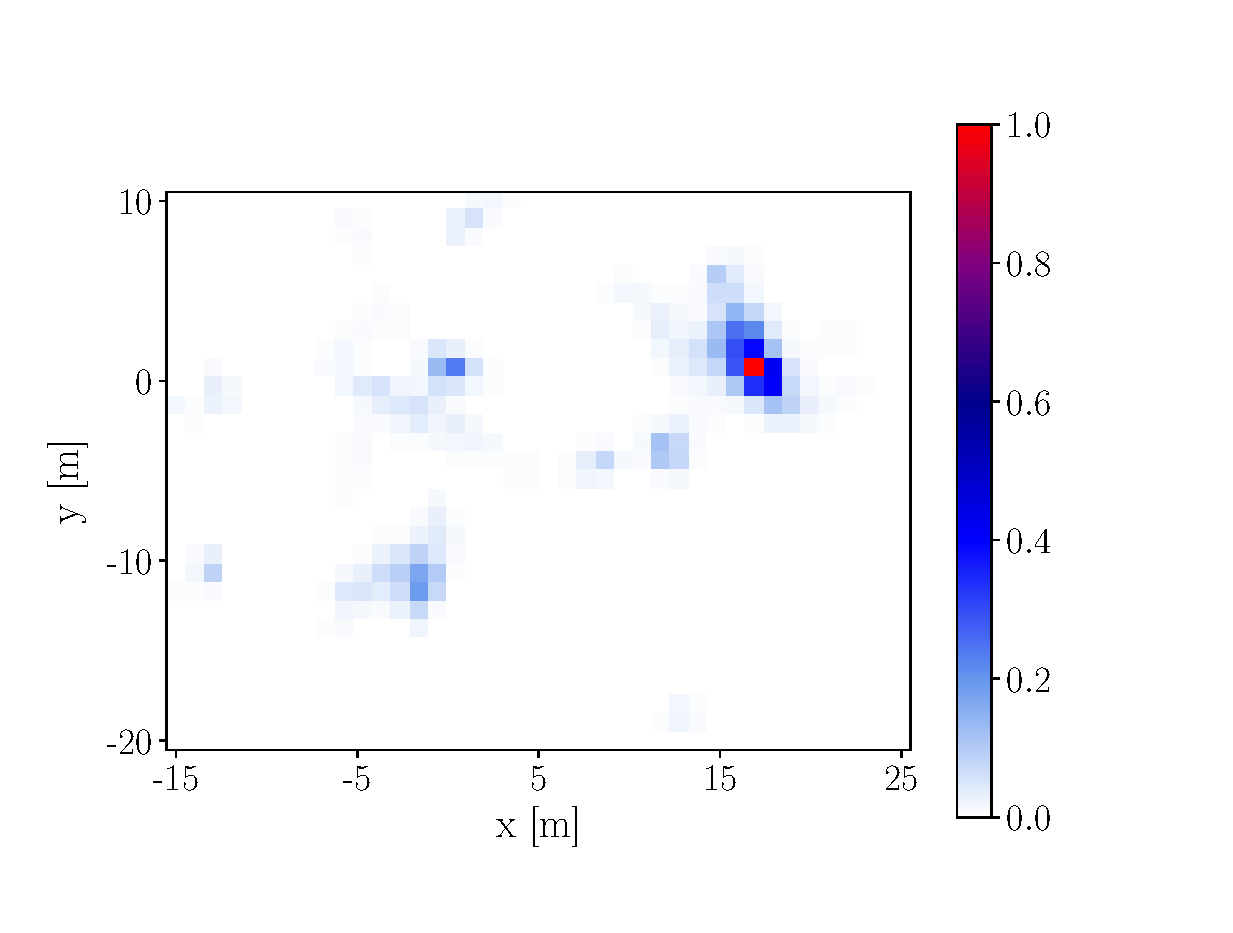
\includegraphics[width=0.5\textwidth,trim={0 0.5cm 2cm 1cm},clip]{./fig/photos/auto_simulation_lam_2.eps}
    \label{e2:lam2}
  }
  \subfloat[($t = \SI{100}{\second}$) sensitivity of detection $\mathbf{s}$ ] {
    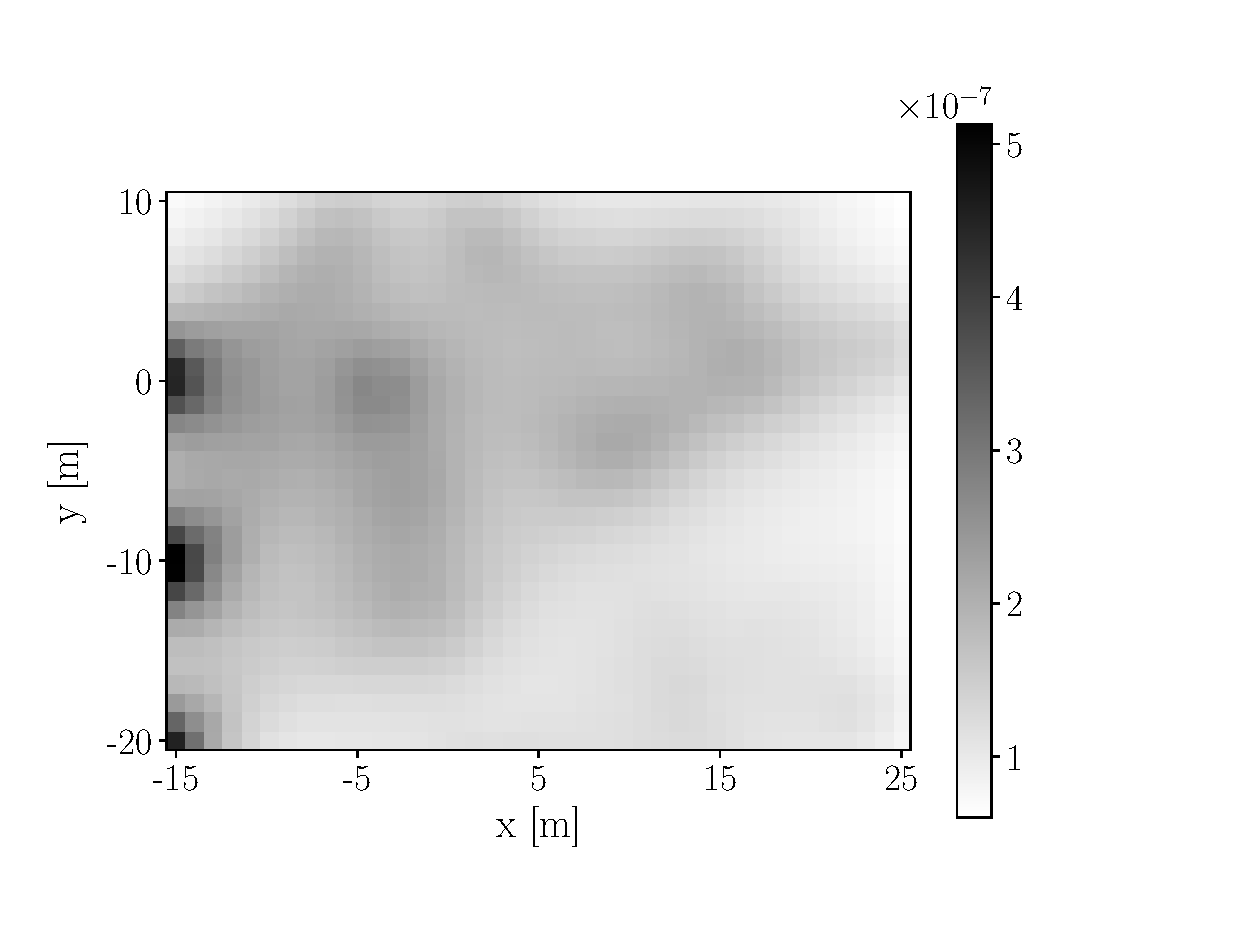
\includegraphics[width=0.5\textwidth,trim={0 0.5cm 2cm 1cm},clip]{./fig/photos/auto_simulation_sen_2.eps}
    \label{e2:sen2}
  }
  \newline
  \noindent
  \subfloat[($t = \SI{100}{\second}$) back projection (number of cones)] {
    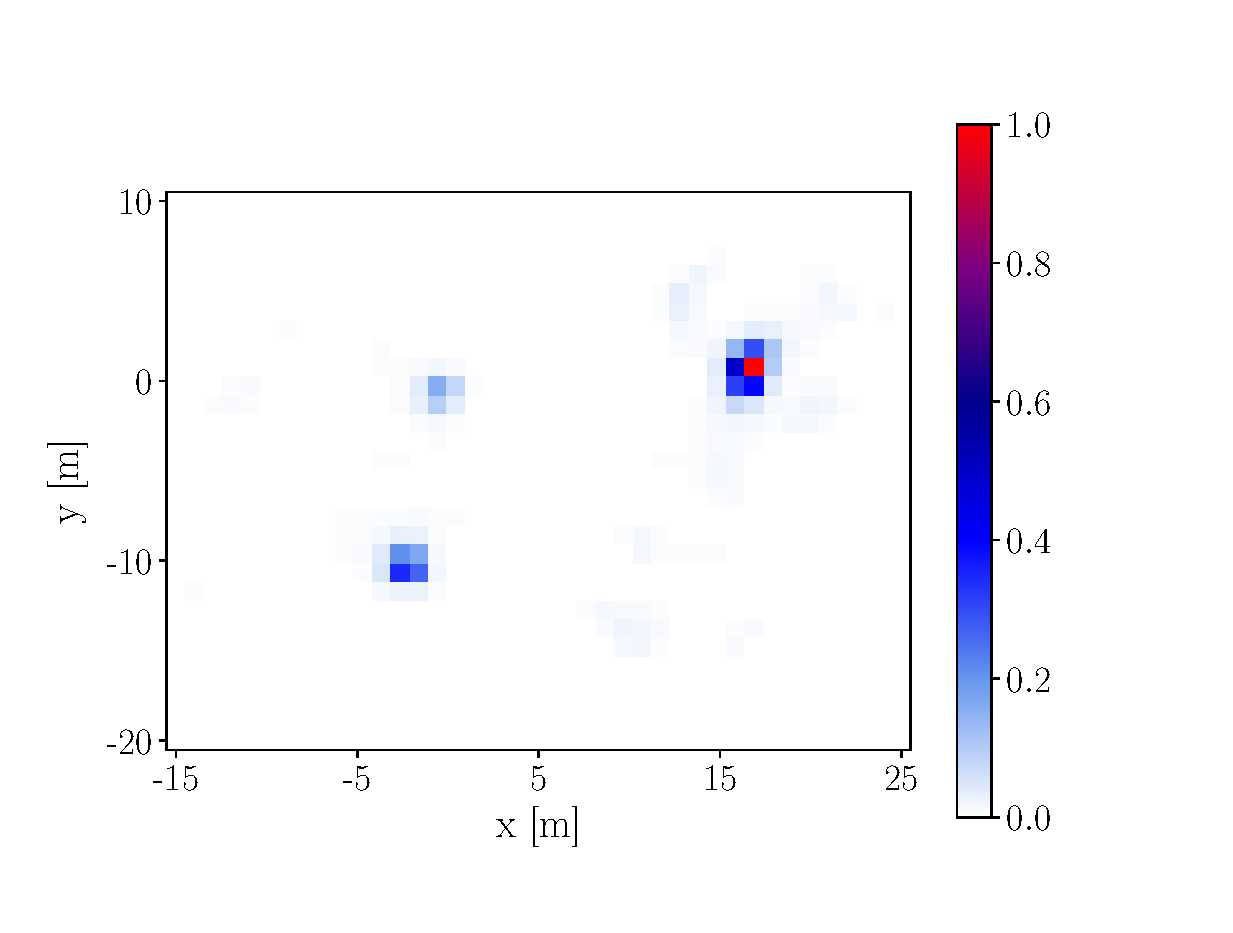
\includegraphics[width=0.5\textwidth,trim={0 0.5cm 2cm 1cm},clip]{./fig/photos/auto_simulation_lam.eps}
    \label{e2:bp}
  }
  \subfloat[ground truth positions of sources ($\si{\mega\becquerel}$)] {
    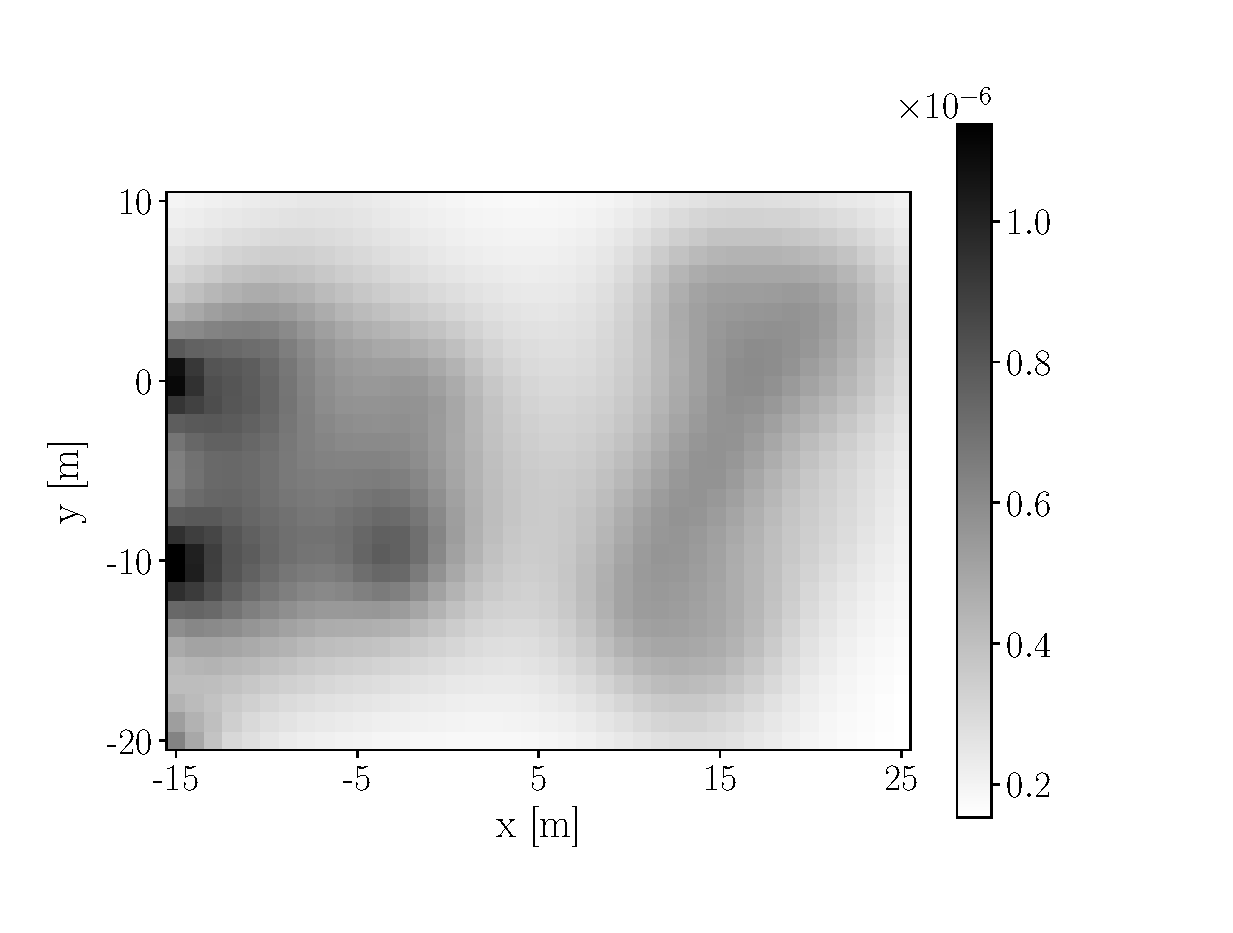
\includegraphics[width=0.5\textwidth,trim={0 0.5cm 2cm 1cm},clip]{./fig/photos/auto_simulation_sen.eps}
    \label{e2:gt}
  }
  \caption{Lorem ipsum}
  \label{fig:e2}
\end{figure}% %%}
}

\subsection{Simulated experiment 2}
The ability to map multiple sources of ionizing radiation is demonstrated on the follwing simulated scenario:
the size of the area, number of drones and other parameters remain the same as in the previous experiment.
Only 
Since the radiation emission is a stochastic process, the same instance was repeated multiple times.




%%%%%%%%%%%%%%%%%%%%%%%%%%%%%%%%%%%%%%%%%%%%%%%%%%%%%%%%%%%%%%%%%%%%%%%
%%%%%%%%%%%%%%%%%%%%%%%%%%%%%%%%%%%%%%%%%%%%%%%%%%%%%%%%%%%%%%%%%%%%%%%%%%
%%%%%%%%%%%%%%%%%%%%%%%%%%%%%%%%%%%%%%%%%%%%%%%%%%%%%%%%%%%%%%%%%%%%%%
\newpage


\section{Real-world experiment with simulated radiation\label{chap:exp3}}
The proposed search strategy has been tested using real \ac{UAV}s during the field experiments.
Since the real sources of radiation were not available, the ionizing radiation was simulated onboard each \ac{UAV}.
The main purpose of the experiment was to test the search strategy with real hardware and gain some experience with real-world conditions, where many things are not as simple as in simulation.
\begin{figure}[!htb]
  \centering
  \subfloat[The DJI f450 drones used during the experiments.] {
    \includegraphics[width=0.5\textwidth]{./fig/photos/experiments.jpg}
    \label{fig:d1}
  }
  \subfloat [The area of interest and \ac{UAV}s searching for the (simulated) sources of ionizing radiation.]{
    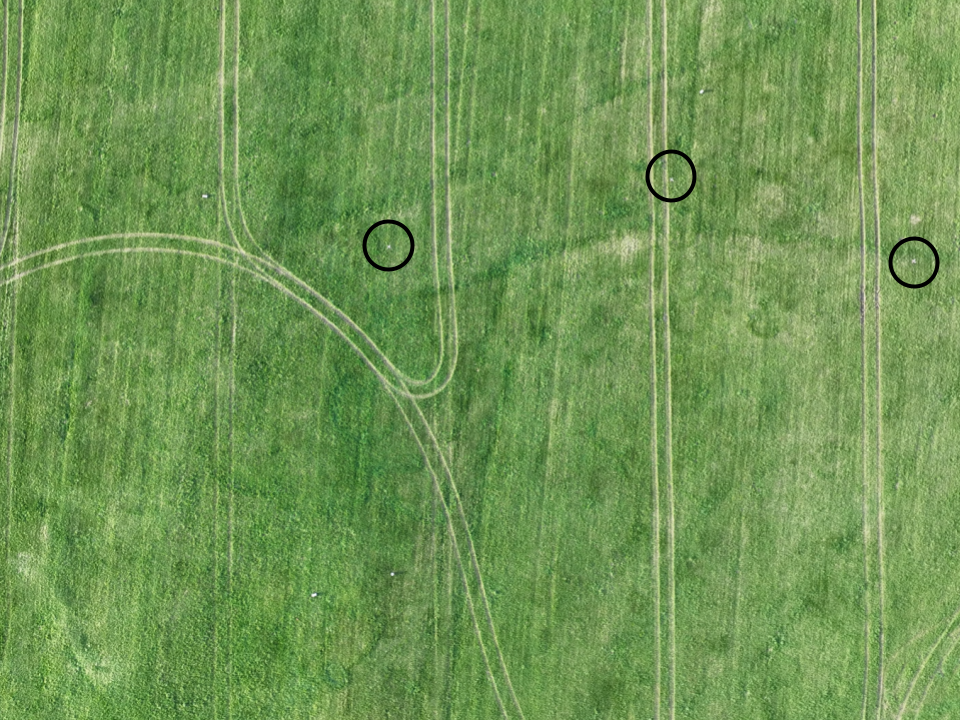
\includegraphics[width=0.5\textwidth]{./fig/photos/pole3.png}
    \label{fig:d2}
  }
  \caption{Field experiments with real hardware. The drones \protect\subref{fig:d1} were mapping the simulated radioactive sources located somewhere in the open field \protect\subref{fig:d2}.}
  \label{fig:}
\end{figure}
\subsection{Experiment setup}
The size of the explored area was $100 \times 100\ \si{\meter}$, the resolution of each map cell was set to $\SI{0.5}{\meter}$.
The simulator of ionizing radiation was running onboard each \ac{UAV}, simulating the radiation coming from sources at predefined positions.
The \ac{UAV}s were localized using \ac{GPS}.
However, the noise in \ac{GPS} position measurement did not affect the simulated radiation data since the drones used their belief (not the real position) when simulating incoming ionizing photons.
The viewpoints (positions of the drones) were sampled with $\SI{5}{\hertz}$, and the \ac{MLEM} estimate was updated every $\SI{2}{\second}$.
Four simulated sources of $\SI{662}{\kilo\electronvolt}$ photons with activity $2000, 1000, 1000, 500\ \si{\mega\becquerel}$ were located at positions shown in  \autoref{e3:gt}.

%The communication between the base station (notebook with \textit{Intel i5-1240P} processor, $\SI{16}{\giga\byte}$ RAM, $\SI{4}{\giga\byte}$ GPU) and the \ac{UAV}s was established via \ac{wifi} network. 

\subsection{Results}
In the initial phase (from time $t = \SI{0}{\minute}$ to time $t = \SI{2}{\minute}$), the drones flew over the area once in a ``zig-zag'' pattern following the predefined trajectory (covering the area uniformly, as can be seen in \autoref{e3:senzig}) and measured first $17$ Compton cones.
The ``zig-zag'' trajectory was precomputed using the MRS UAV System \cite{mrs_system}.
The \ac{MLEM} estimate and sensitivity of detection after the initial phase is shown in \autoref{e3:lamzig} and \autoref{e3:senzig}.
Then (at the time $t = \SI{2}{\minute}$), the proposed search strategy took control---two drones were designated for exploitation, one for exploration.
The trajectories of the \ac{UAV}s during the search phase (\autoref{e3:paths}) show that the two ``exploitation`` drones focused on acquiring more measurements while the third drone was exploring the unexplored area.
The final estimate of radiation sources intensities (at the end of the experiment $t = \SI{10}{\minute}$) is shown in \autoref{e3:lam}.
Three of four sources of simulated ionizing radiation were correctly localized (together with their relative emission activity, which is shown in table \autoref{tab:temenight_results}).
The weakest $\SI{500}{\mega\becquerel}$ source at position ($75, 75$) was not discovered despite the fact that the exploration drone flew around it multiple times (see blue path in \autoref{e3:paths}).
The minimum distance between the \ac{UAV}s was not below the safety threshold ($\SI{4}{\meter}$) during the whole flight, therefore all the planned trajectories were non-colliding.
267 Compton events were recorded during the whole experiment.
\begin{table}[htb]
\begin{center}
  \begin{tabular}{ |c|c|c|c| } 
 \hline
    \multicolumn{2}{|c}{Sources} &  \multicolumn{2}{|c|}{ relative activity } \\
 \hline
    position & activity & ground truth & MLEM estimate\\ 
 \hline
    (10, 20) & 2000 MBq & 1.0  & \textbf{1.0} \\ 
    (20, 20) & 1000 MBq &  0.5 & \textbf{0.49} \\ 
    (80, 80) & 1000 MBq &  0.5 & \textbf{0.52} \\ 
    (75, 75) & 500 MBq &  0.25 & \textbf{0.0} \\ 
 \hline
\end{tabular}
  \caption{Results of the real-world experiment with simulated data. The last column presents estimated relative activity at the map positions that correspond to the ground truth position of the given source.}
  \label{tab:temenight_results}
\end{center}
\end{table}

\subsection{Summary}
The experiment proved that the whole system be used for fast radiation mapping in large open areas and perform all the computations in real-time.
The proposed search strategy, together with the \ac{MLEM} mapping method, worked as intended.
The initial estimate of source positions was significantly improved during the search phase.
Although the maximum likelihood does not provide an accurate estimate for a small number of cones (see \ac{MLEM} estimate in \autoref{e3:lamzig} generated from 17 Compton cones), the inaccurate estimate ``attracts'' the \ac{UAV}s that come closer and likely measure more ionizing photons, that guide the \ac{UAV}s to the actual position of the source.
This shows that online estimation (together with an active search strategy) is beneficial for the autonomous detection of ionizing radiation.

Three of four sources of simulated radiation were localized during the experiment.
The weakest $\SI{500}{\mega\becquerel}$ was not discovered during the flight, which is probably caused more by the limited sensitivity of the (simulated) \ac{pix} sensor than by the estimation method. It is important to note that the simulated radiation data were generated in ideal conditions, without any noise in the drone position, energies measured in the sensor or particles causing false positive Compton detections.
Therefore the results of \ac{MLEM} reconstruction results are more accurate compared to the previously described experiments with real sources of ionizing radiation.

% Answer: [trim={left bottom right top},clip]
% Ex. 1: trim from left edge
%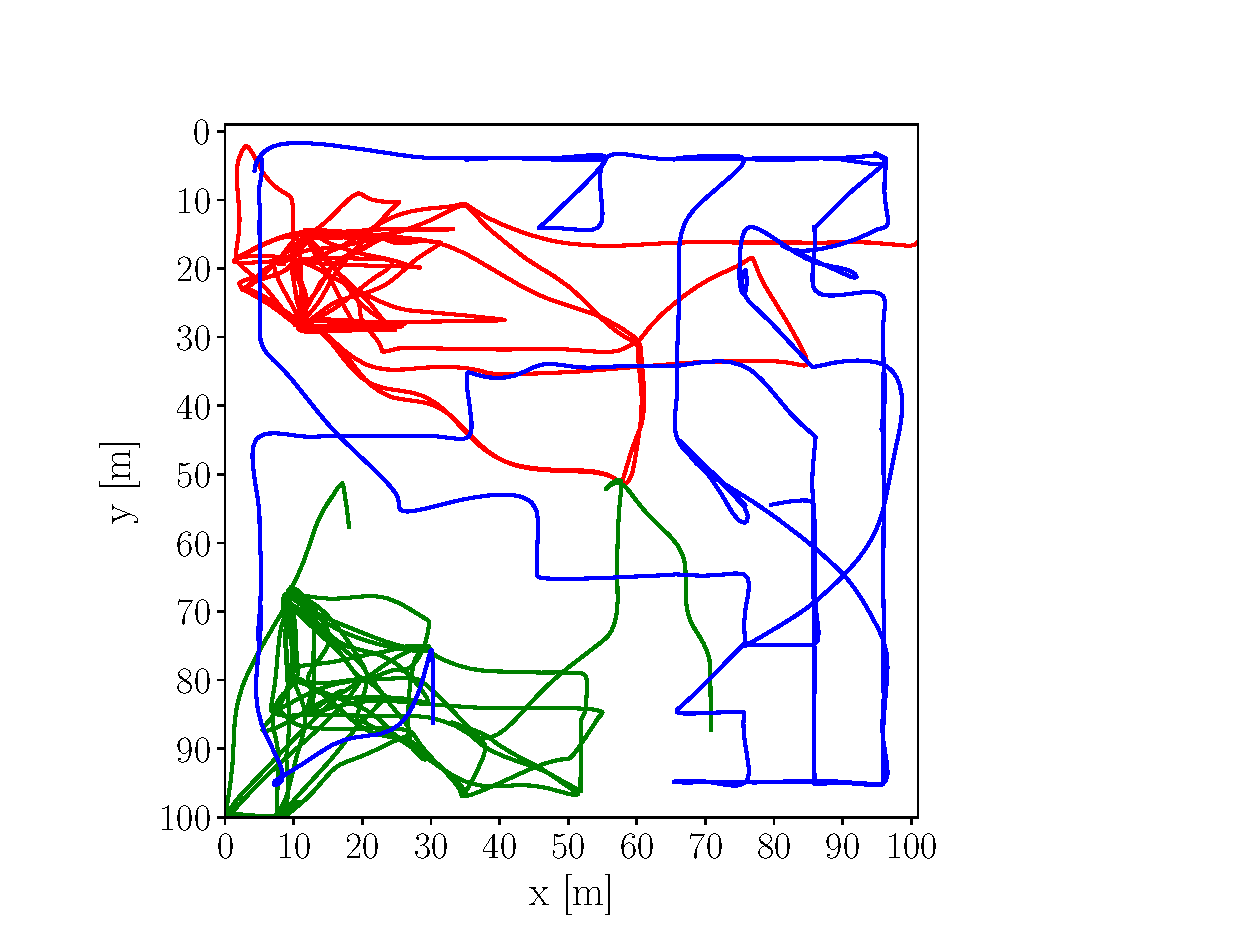
\includegraphics[width=0.5\textwidth,trim={0 0 2cm 2cm},clip]{./fig/photos/auto_temesvar_drone_paths.eps}


\begin{figure}[ht!]% %%{
  \centering
  
  \subfloat[source intensities $\bm{\lambda}$ after the initial phase ($t = \SI{2}{\minute}$) ] {
    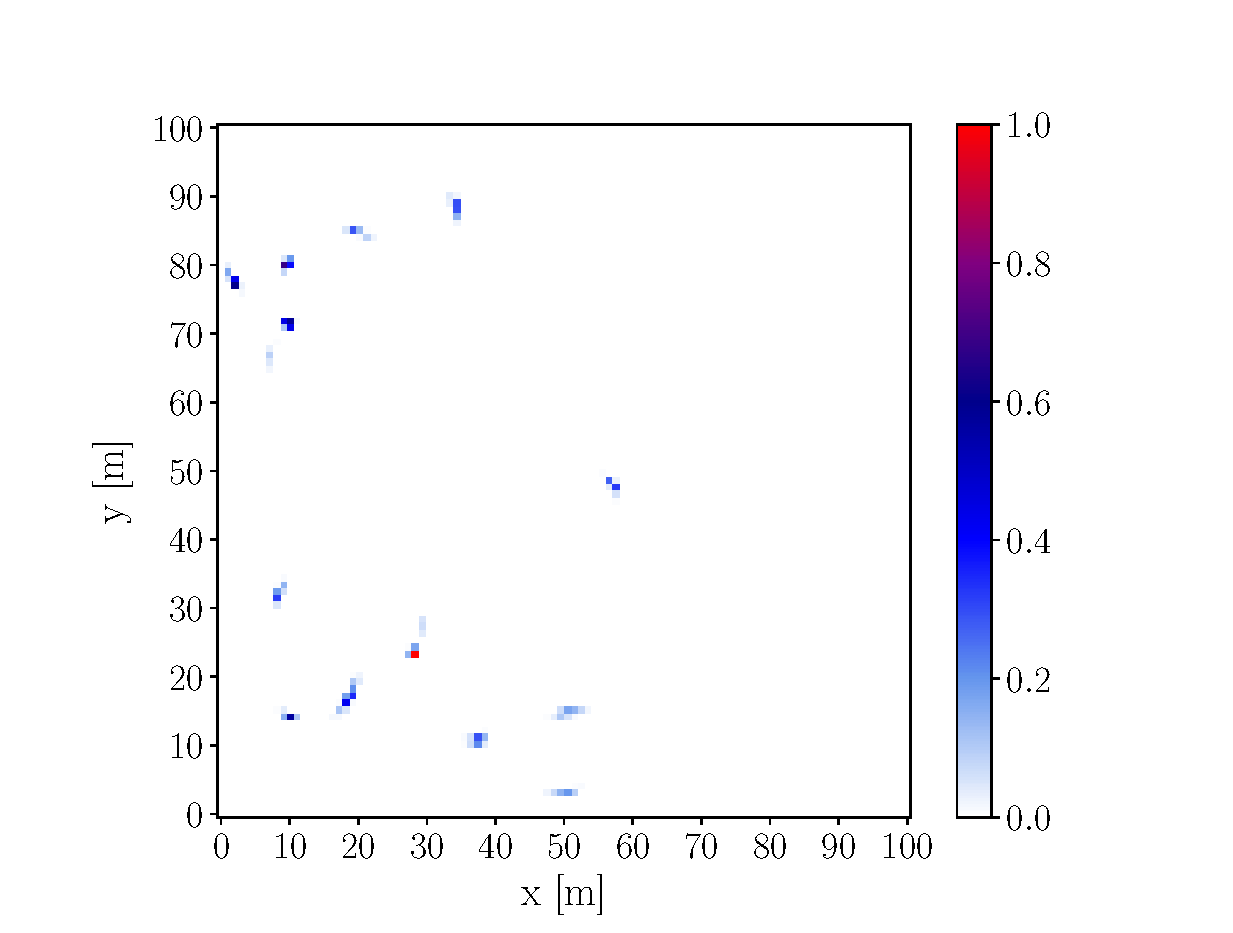
\includegraphics[width=0.5\textwidth,trim={1cm 0 2.5cm 1.2cm},clip]{./fig/photos/auto_temesvar_lamzig.eps}
    \label{e3:lamzig}
  }
  \subfloat[Sensitivity $\mathbf{s}$ after the initial phase ($t = \SI{2}{\minute}$)] {
    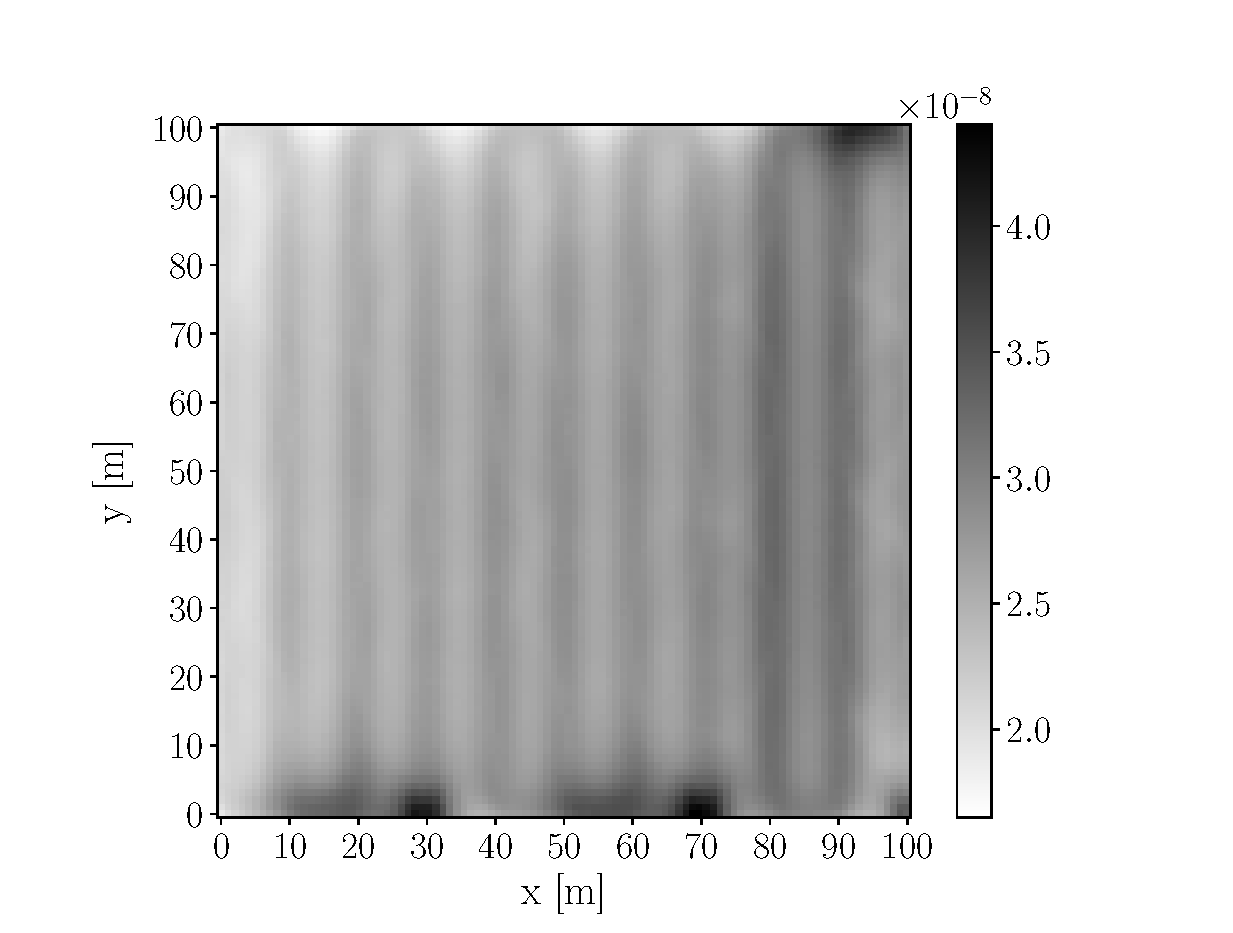
\includegraphics[width=0.5\textwidth,trim={1cm 0 2.5cm 1.2cm},clip]{./fig/photos/auto_temesvar_senzig.eps}
    \label{e3:senzig}
  }
  \newline
  \noindent 
  \subfloat[final estimate of source intensities $\bm{\lambda}$($t = \SI{10}{\minute}$)] {
    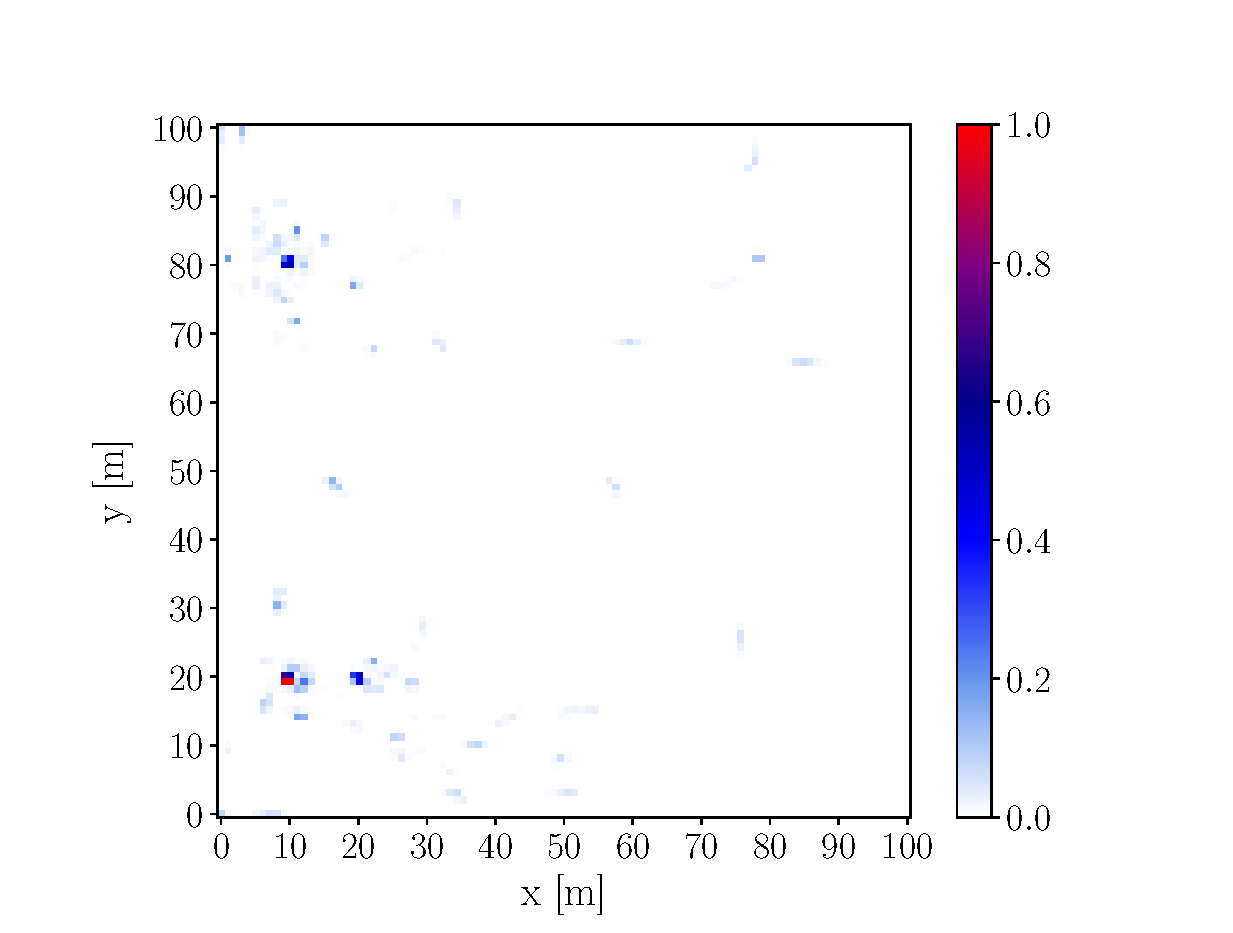
\includegraphics[width=0.5\textwidth,trim={1cm 0 2.5cm 1.2cm},clip]{./fig/photos/auto_temesvar_lam.eps}
    \label{e3:lam}
  }
  \subfloat[Sensitivity $\mathbf{s}$ at the end of the experiment ($t = \SI{10}{\minute}$)] {
    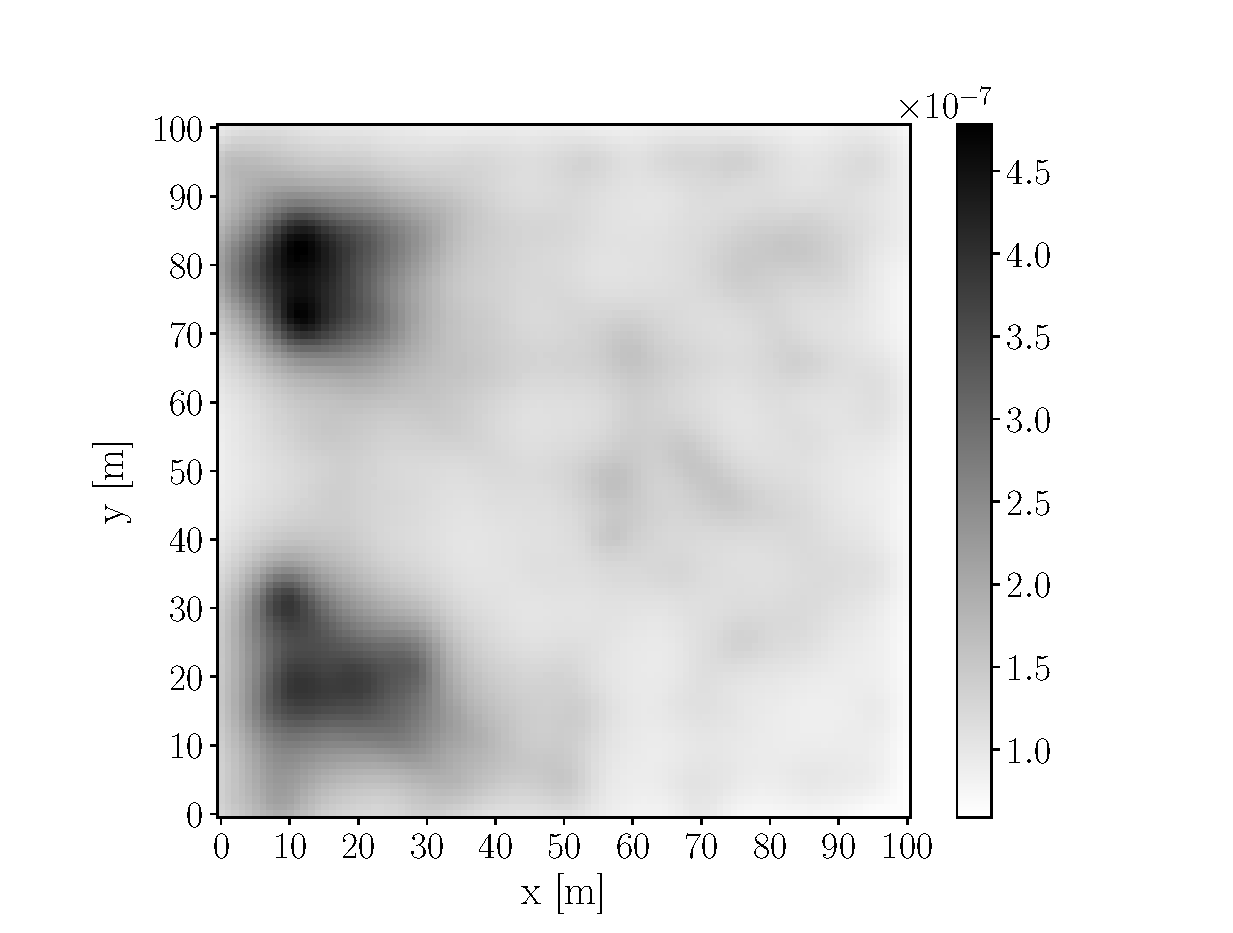
\includegraphics[width=0.5\textwidth,trim={1cm 0 2.5cm 1.2cm},clip]{./fig/photos/auto_temesvar_sen.eps}
    \label{e3:sen}
  }
  \newline
  \noindent 
  \subfloat[ground truth ($\si{MBq}$)] {
    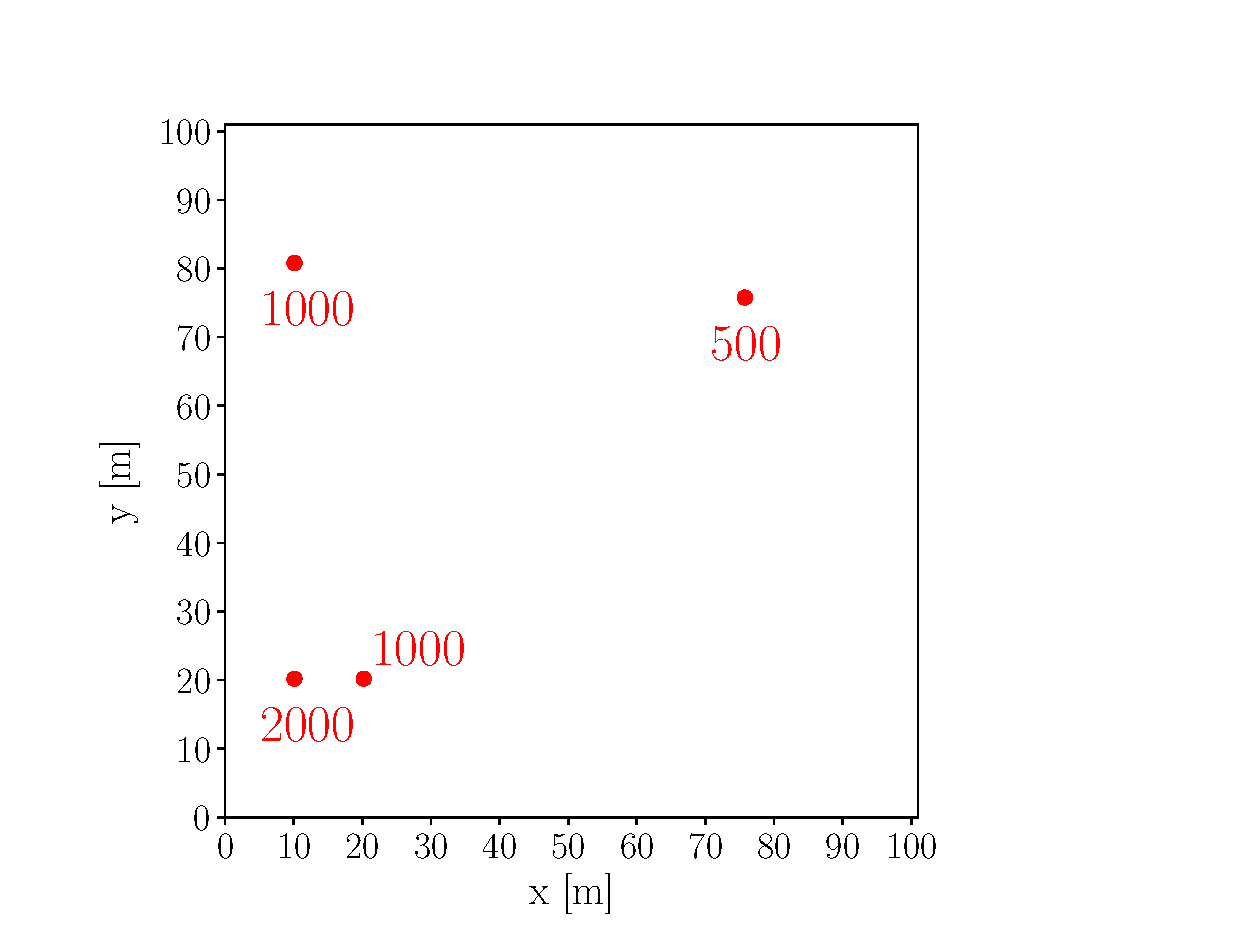
\includegraphics[width=0.5\textwidth,trim={1cm 0 2.5cm 1.7cm},clip]{./fig/photos/auto_temesvar_gt.eps}
    \label{e3:gt}
  }
  \subfloat[Paths of \ac{UAV}s during the search phase \newline (red, green --- exploitation, blue --- exploration)] {
    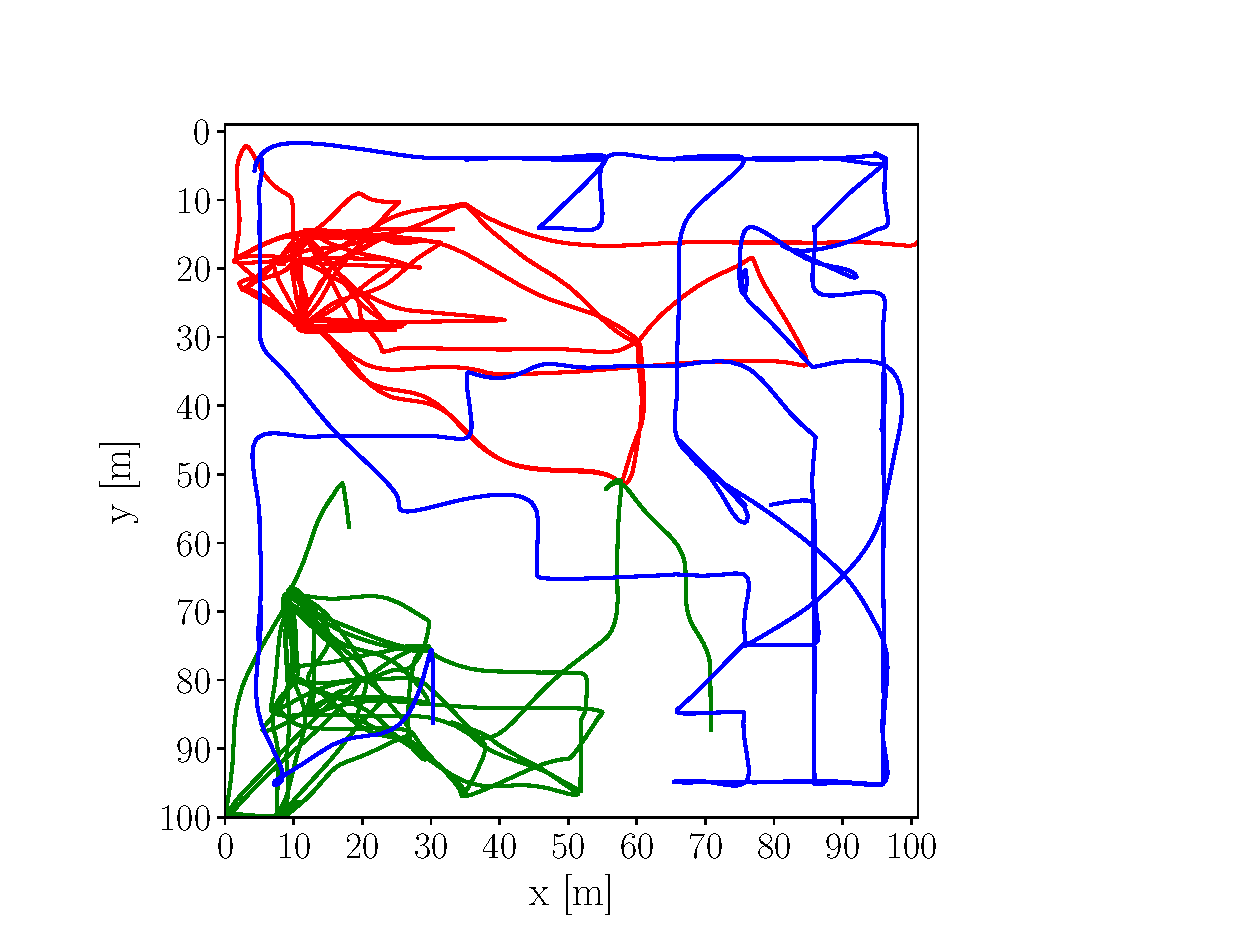
\includegraphics[width=0.5\textwidth,trim={1cm 0 2.5cm 1.7cm},clip]{./fig/photos/auto_temesvar_drone_paths.eps}
    \label{e3:paths}
  }
  %\subfloat[Final back-propagation.] {
  %  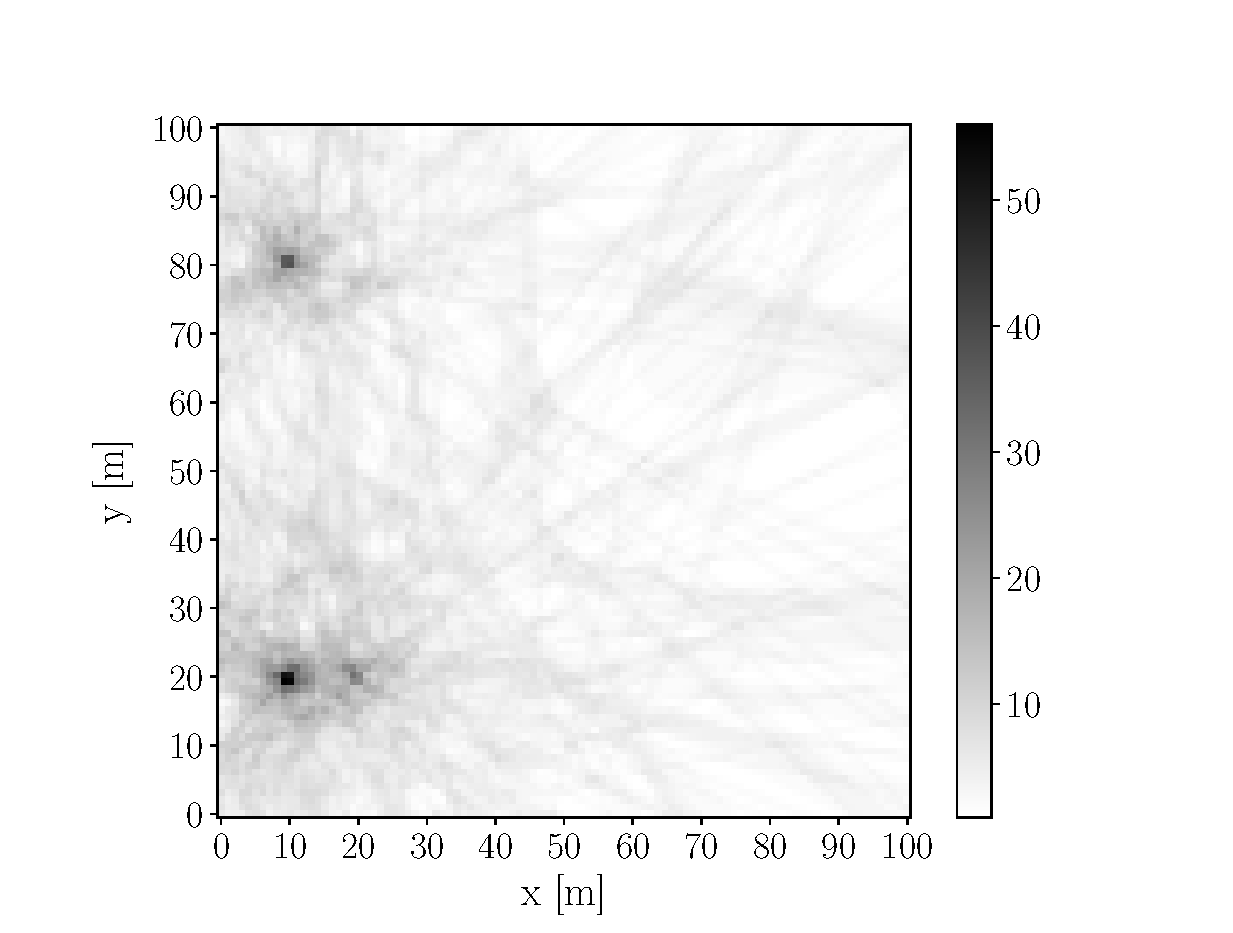
\includegraphics[width=0.5\textwidth,trim={1cm 0 2.5cm 1cm},clip]{./fig/photos/auto_temesvar_bp.eps}
  %  \label{e3:bp}
  %}
  \label{fig:e3}
  \caption{Real-world experiments with simulated data. The \ac{MLEM} estimate, sensitivity and drone paths during and after the experiment ($t = \SI{2}{\minute}$, $t = \SI{10}{\minute}$) are presented.}
\end{figure}% %%}



\mycomment{% %%{

\section{Monte carlo simulation results}
In \autoref{fig:monte_cs_results}, the probability of a Cesium-137 photon generating a Compton cone when emitted from a distance of 1 meter is displayed. 
The sensor's sensitivity is observed to be nearly uniform regardless of the incoming particle's direction. 
This outcome can be explained using \autoref{fig:monte_clar}. 
As illustrated in \autoref{fig:monte_reaching}, particles that approach the sensor from the front side have a greater visible surface area, resulting in a greater likelihood of hitting the sensor. 
Conversely, particles arriving from the side have a longer intersection with the sensor's material, resulting in a greater probability of producing a Compton cone, as shown in  \autoref{fig:monte_cone_from_hitting}. 
Surprisingly, these two effects compensate for each other, resulting in an almost consistent sensitivity of the sensor to particles arriving from various directions.

\begin{figure}[!htb]
  \centering
  \subfloat {
    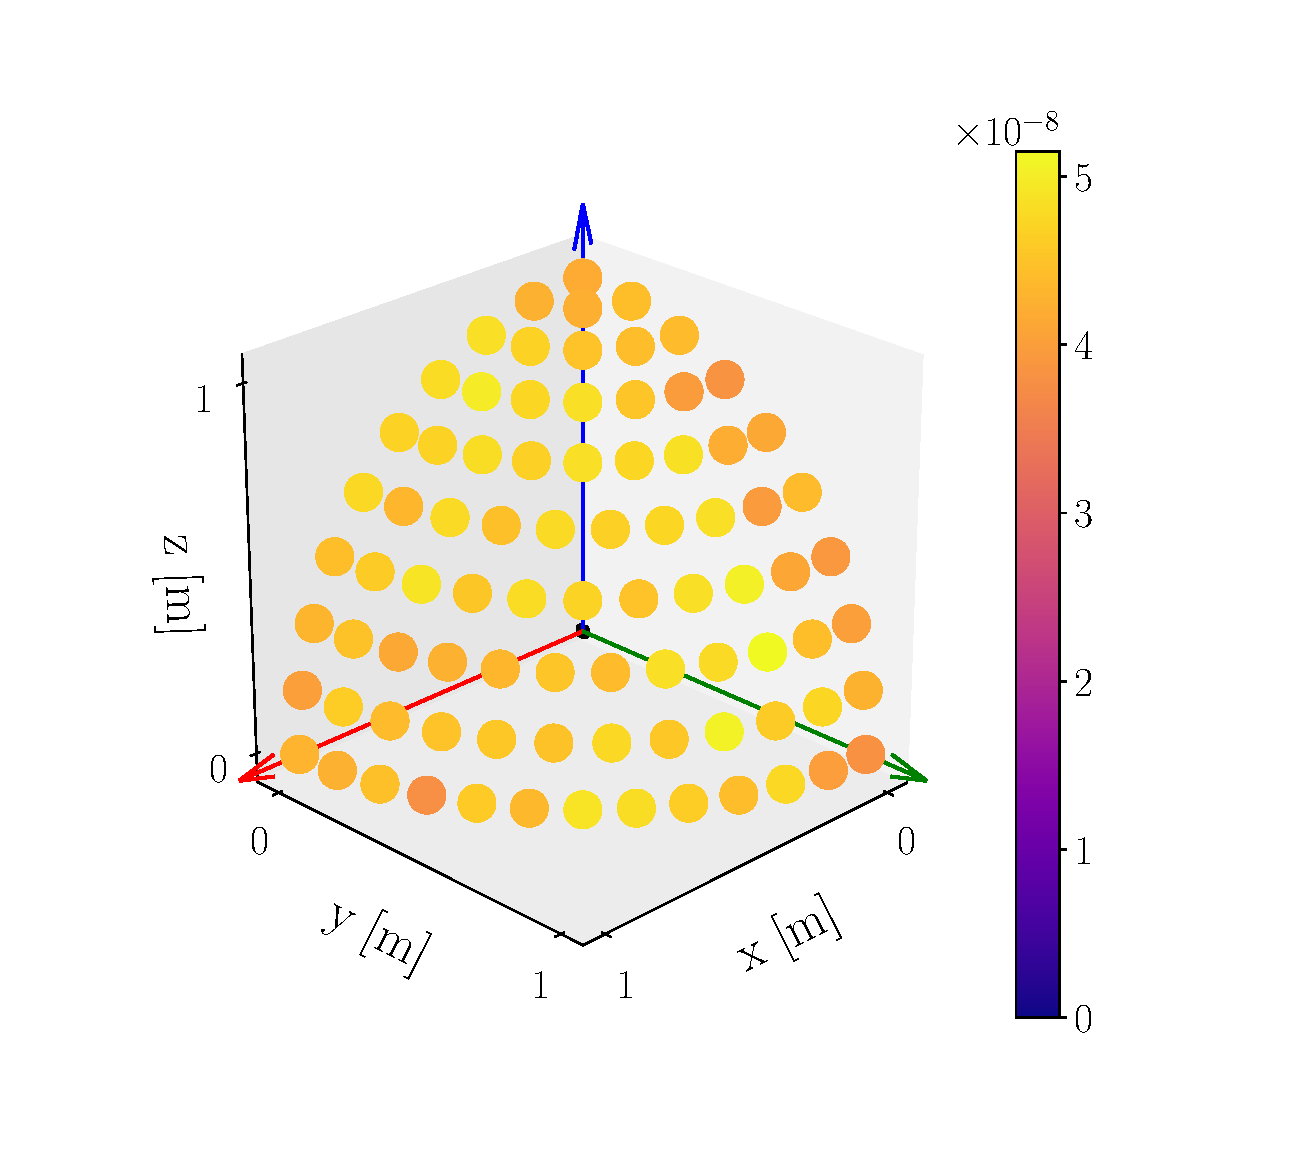
\includegraphics[width=0.7\textwidth]{./fig/photos/monte_carlo_final_prob.eps}
  }
  \caption{$p(\mathrm{cone\ detected})$ - probability that particle emitted at certain position produces a compton cone.}
  \label{fig:monte_cs_results}
\end{figure}


\section{Evaluation on recorded real-world data}
TODO
\section{Simulations in gazebo}

\section{Real-world experiment with simulated sources}

\subsection{Experimental setup}
The radiation mapping pipeline was tested on a real hardware during the field experiments.
Three \ac{UAV} were used during this experiment.
The real radioactive sources were replaced with simulated ones, the Compton camera simulator \cite{TODO} was running onboard each \ac{UAV}.
All the drones were localized using \ac{gps} in the same coordinate frame and the positions of simulated sources were shared among them.
The size of mapped area was set to $100 \times 100$ m, four simulated sources with activities 500 MBq, 1 GBq, 2 GBq and 2 GBq were placed in the area.
Resolution of the map was $0.5$ m.

\subsection{Results}
\begin{table}[htb]
\begin{center}
  \begin{tabular}{ |c|c|c|c| } 
 \hline
    \multicolumn{2}{|c}{Sources} &  \multicolumn{2}{|c|}{ relative activity } \\
 \hline
    position & activity & ground truth & MLEM estimate\\ 
 \hline
    (10, 20) & 2000 MBq & 1.0  & \textbf{1.0} \\ 
    (20, 20) & 1000 MBq &  0.5 & \textbf{0.49} \\ 
    (80, 80) & 1000 MBq &  0.5 & \textbf{0.52} \\ 
    (75, 75) & 500 MBq &  0.25 & \textbf{0.0} \\ 
 \hline
\end{tabular}
  \caption{Results of the real world experiment with simulated data. Last column presents estimated relative activity at the map positions that correspond to the ground truth position of the given source.}
  \label{tab:temenight_results}
\end{center}
\end{table}

% Answer: [trim={left bottom right top},clip]
% Ex. 1: trim from left edge


\begin{figure}[!htb]
  \centering
  \subfloat {
    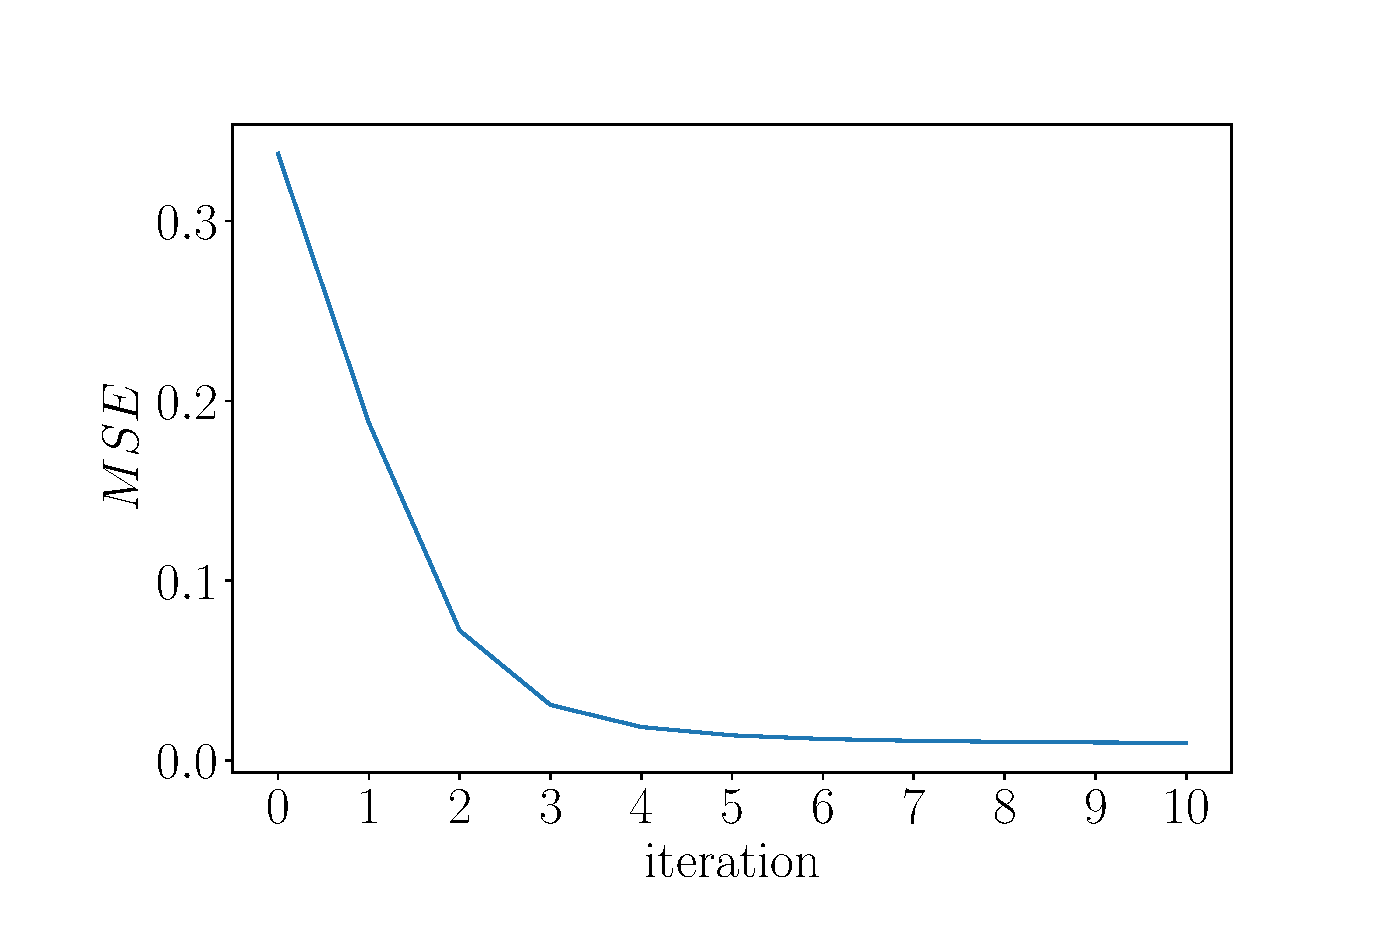
\includegraphics[width=0.7\textwidth]{./fig/photos/auto_mse_realworld.eps}
  }
  \caption{$p(\mathrm{cone\ detected})$ - probability that particle emitted at certain position produces a compton cone.}
  \label{fig:monte_cs_results}
\end{figure}


}% %%}

\mycomment{% %%{
    This describes experiments and evaluation of performance of the proposed method for mapping of ionizing radiation.
    An experiment with real sources of ionizing radiation requires (due to specific safety measures, permission from the state authorities...) coordination with other institutions, such as Czech metrology institute.
    Unfortunately, it was not possible to perform experiment with real sources before the deadline of the thesis due to these organizational reasons.
    However, the method was evaluated on pre-recorded data from real-world experiments as well as using the realistic simulator for compton camera \cite{TODO}.
}% %%}

\mycomment{% %%{




    \section{Pre-recorded data with real radioactive sources}


    \section{Gazebo simulations with the simulated Compton camera}

    \section{Real-world experiment with the simulated Compton camera}



    The approach presented in the previous was applied on a prerecorded rosbag from a real-world experiment.
    Four \ac{UAV}s were used in this experiment.
    The mapped area was $50 \times 35$ meters with $0.4$ m resolution.
    The experiment took approximately 8 minutes and 250 cones were measured.

    The estimated vector of $\bf{\lambda}$ is presented in \autoref{fig:D}. 
    The ground truth positions of radioactive sources with their strength can be seen on \autoref{fig:C}.
    The sensitivity vector $\mathbf{s}$ and the matrix $\mathbf{T}$ summed over all measurements (which serves as simple projection of the cones to the map) are presented in  \autoref{fig:E} and \autoref{fig:F}.

    \begin{figure}[!h]
      \centering
      \subfloat[True positions of sources (MBq)] {
        
\includegraphics[width=0.5\textwidth]{./fig/photos/temenight_ground_truth.eps}
        \label{fig:C}
      }
      \subfloat[MLEM estimate after 10 iterations] {
        
\includegraphics[width=0.5\textwidth]{./fig/photos/temenight_lambdas.eps}
        \label{fig:D}
      }
      \label{fig:A}
      \caption{Comparison of \ac{MLEM} algorithm estimate and the ground truth.}
    \end{figure}

    \begin{figure}[!htb]
      \centering
      \subfloat[System matrix $\mathbf{T}$ summed over $\forall i$] {
        
\includegraphics[width=0.5\textwidth]{./fig/photos/temenight_back_projection.eps}
        \label{fig:E}
      }
      \subfloat[Sensitivity vector $\mathbf{s}$] {
        
\includegraphics[width=0.5\textwidth]{./fig/photos/temenight_sensitivity.eps}
        \label{fig:F}
      }
      \label{fig:B}
      \caption{System matrix and sensitivity vector estimated during the experiment}
    \end{figure}

    \section{Discussion}
    We can see that the algorithm precisely detected the 500 MBq source. Two smallest source were not recognised, probably due to low number of cones measured.
    The 1900 MBg source was partially detected. 
    In is important to note that the drones were flying mostly around the 500 MBg source and most of the measured cones originated from that source, as we can see in the sensitivity vector and system matrix.
    This approach seems to be beneficial compared to naive back-projection of the cones to the map (without weighting with the sensitivity), since it can "see" the 1900 MBq source despite the fact that only few cones originated there.

\begin{figure}[!htb]% %%{
  \centering
  \subfloat[estimate of sources locations $\bm{\lambda}$ (rescaled)] {
    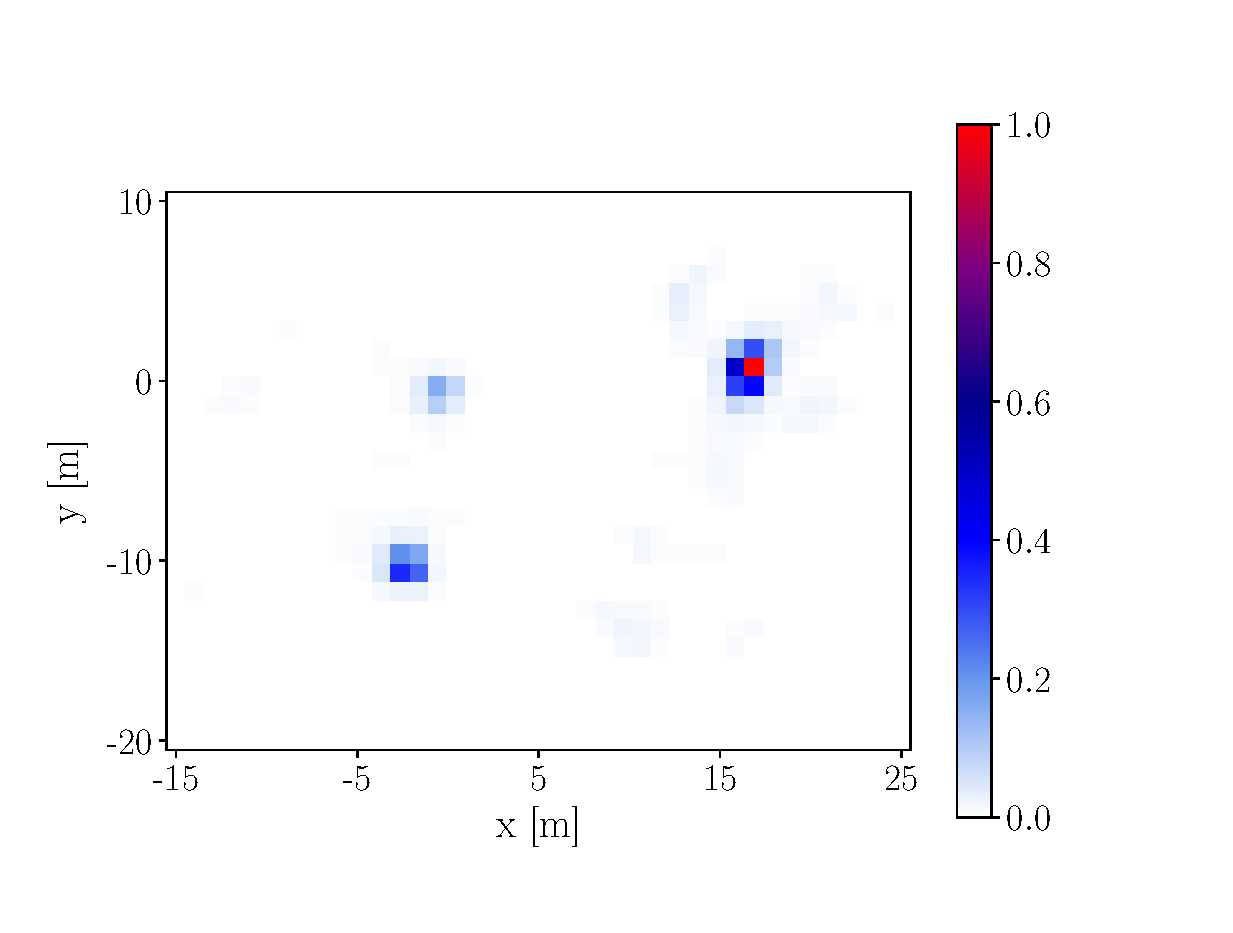
\includegraphics[width=0.5\textwidth,trim={0 0.5cm 2cm 1cm},clip]{./fig/photos/auto_simulation_lam.eps}
    \label{fig:}
  }
  \subfloat[ground truth positions of sources ($\si{\mega\becquerel}$)] {
    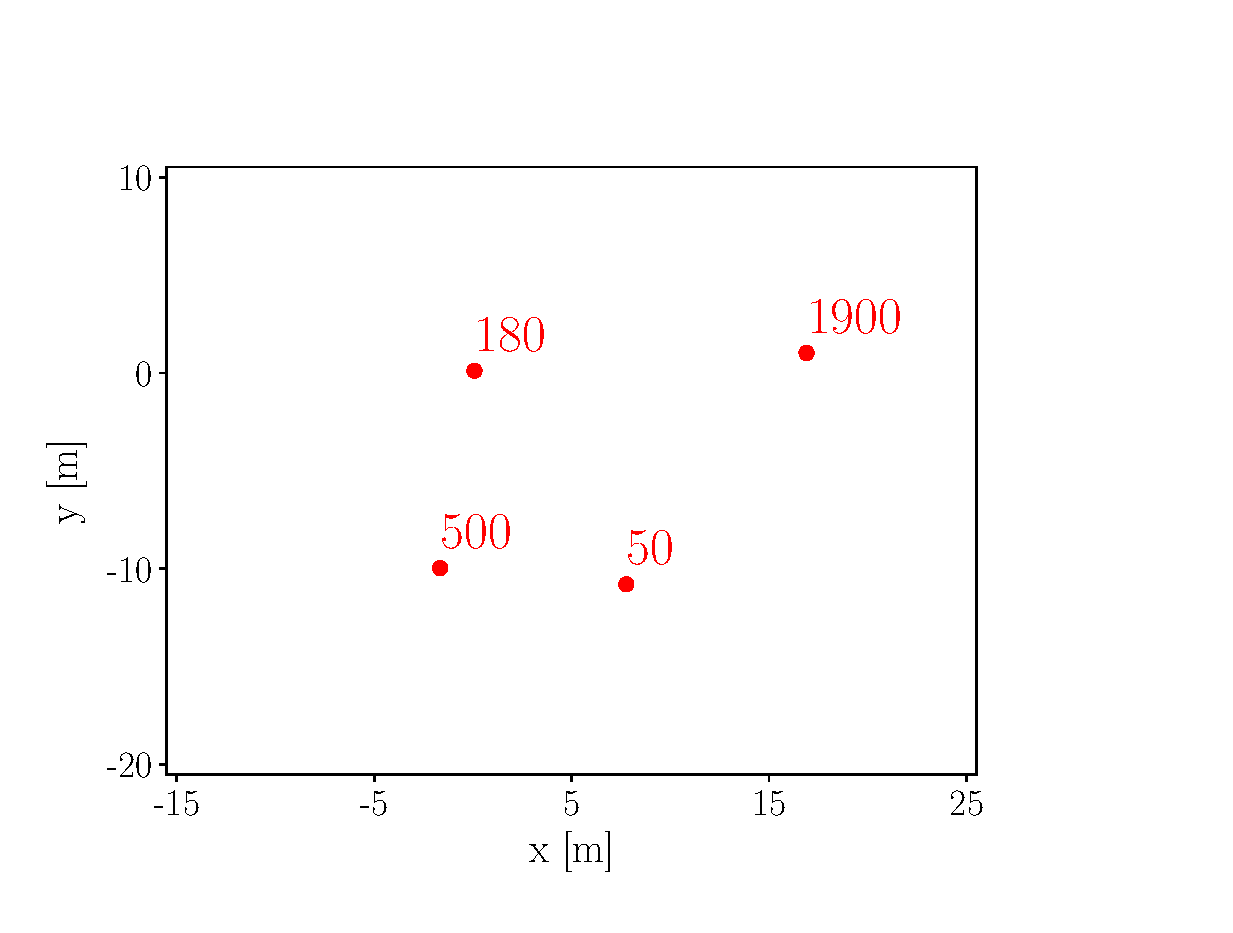
\includegraphics[width=0.5\textwidth,trim={0 0.5cm 2cm 1cm},clip]{./fig/photos/auto_simulation_gt.eps}
    \label{fig:}
  }
  \newline
  \noindent 
  \subfloat[back projection (number of Compton cones)] {
    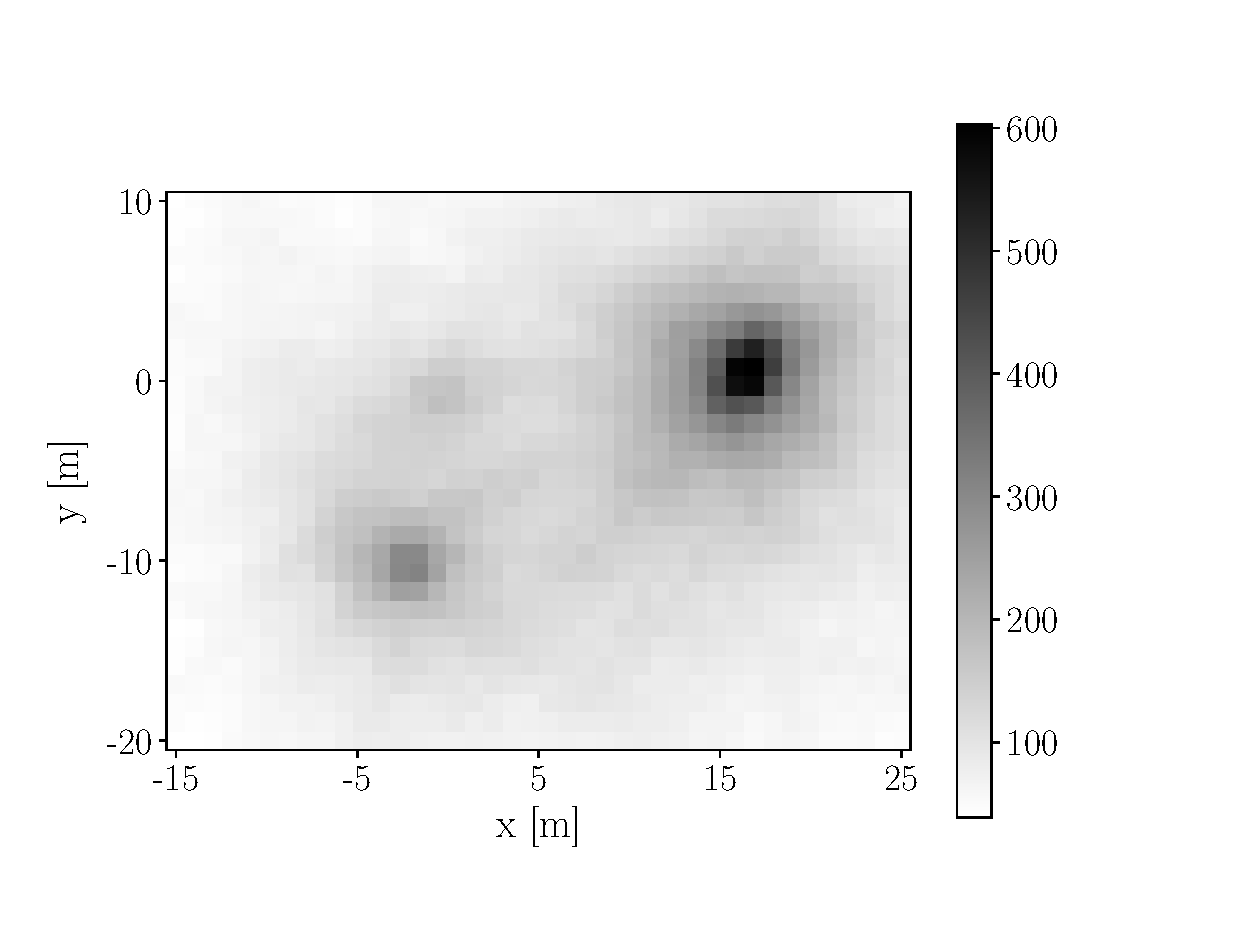
\includegraphics[width=0.5\textwidth,trim={0 0.5cm 2cm 1cm},clip]{./fig/photos/auto_simulation_bp.eps}
    \label{fig:}
  }
  \subfloat[sensitivity of detection $\mathbf{s}$] {
    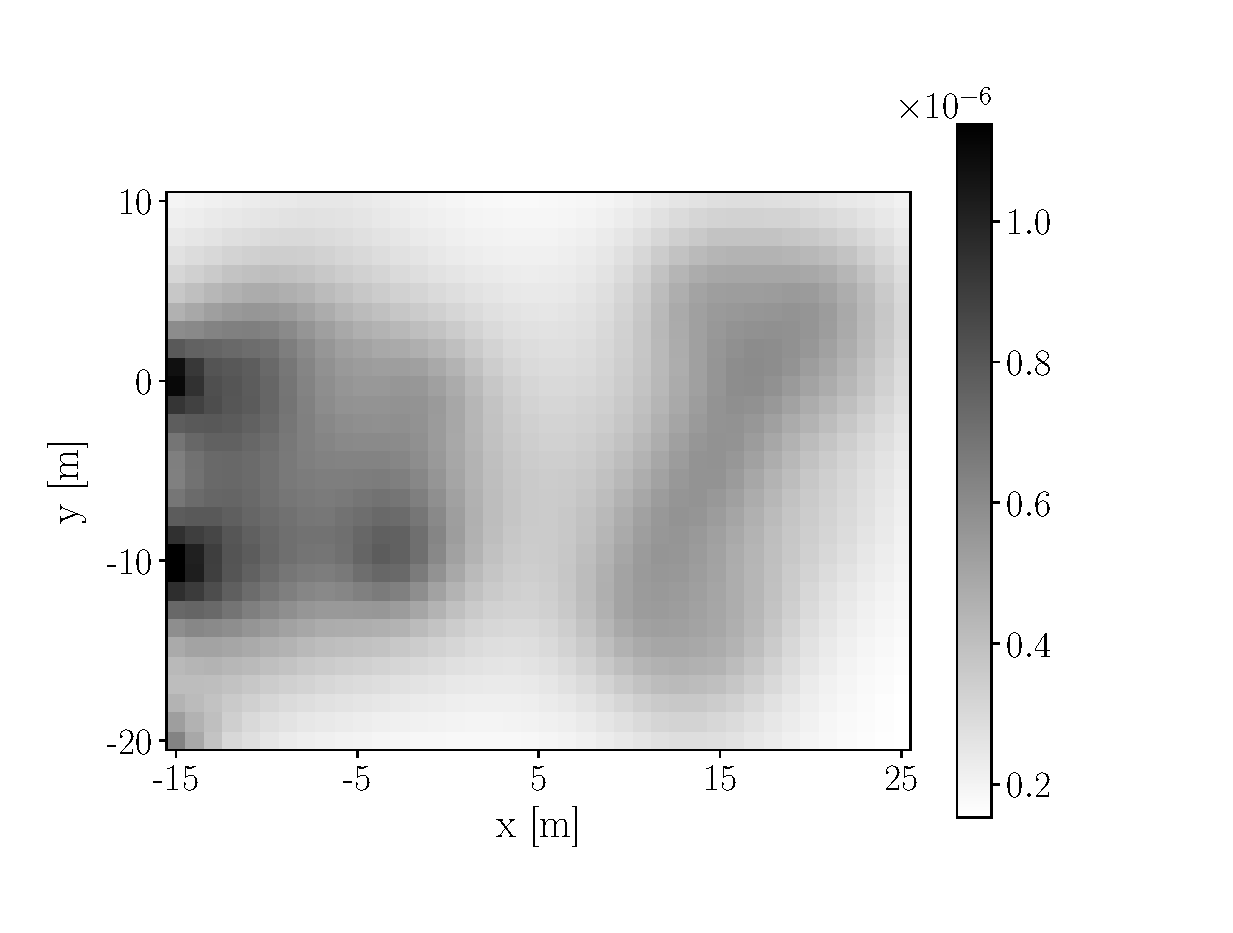
\includegraphics[width=0.5\textwidth,trim={0 0.5cm 2cm 1cm},clip]{./fig/photos/auto_simulation_sen.eps}
    \label{fig:}
  }
  \newline
  \noindent 
  \subfloat[sensitivity of detection $\mathbf{s}$] {
    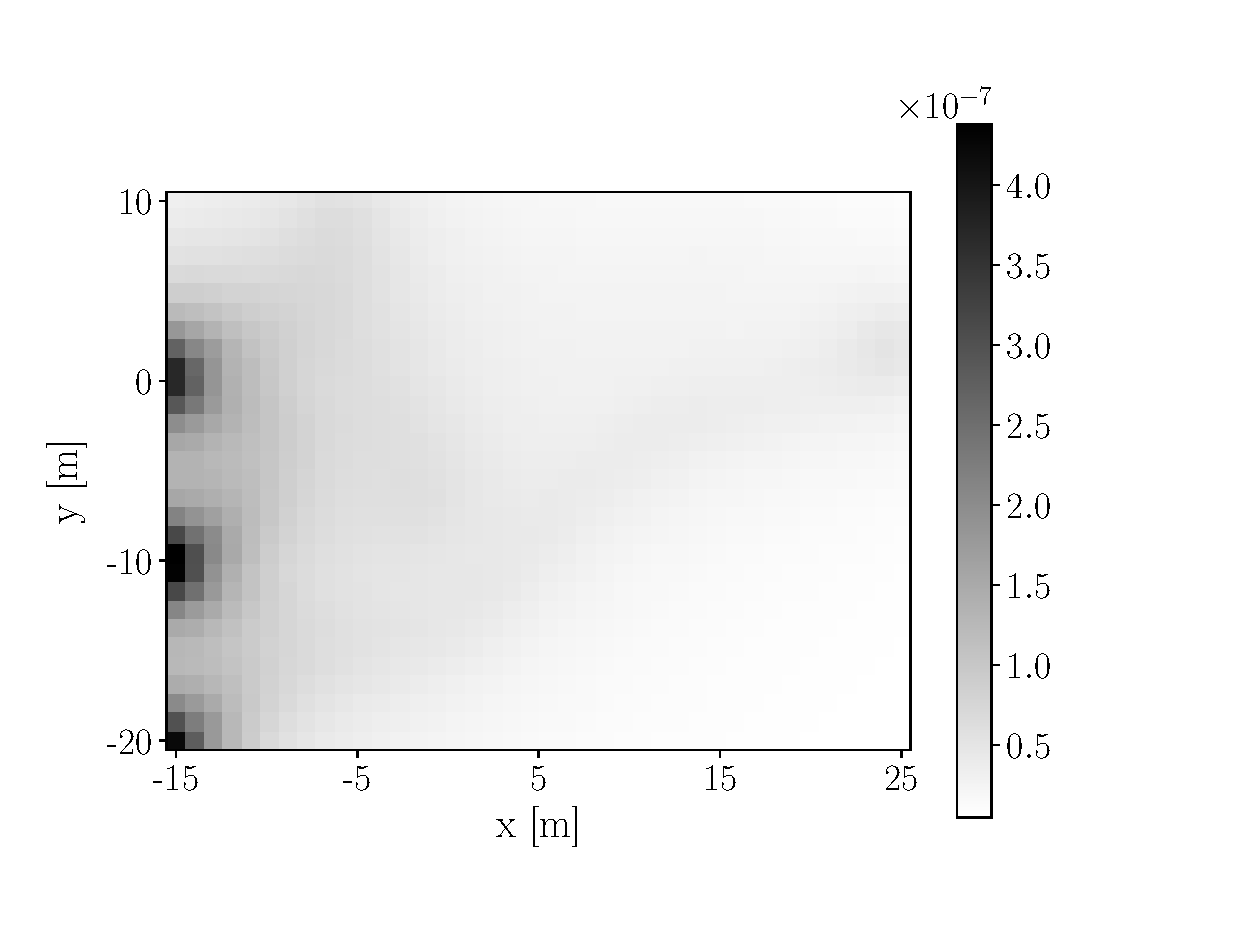
\includegraphics[width=0.5\textwidth,trim={0 0.5cm 2cm 1cm},clip]{./fig/photos/auto_simulation_sen_1.eps}
    \label{fig:}
  }
  \subfloat[sensitivity of detection $\mathbf{s}$] {
    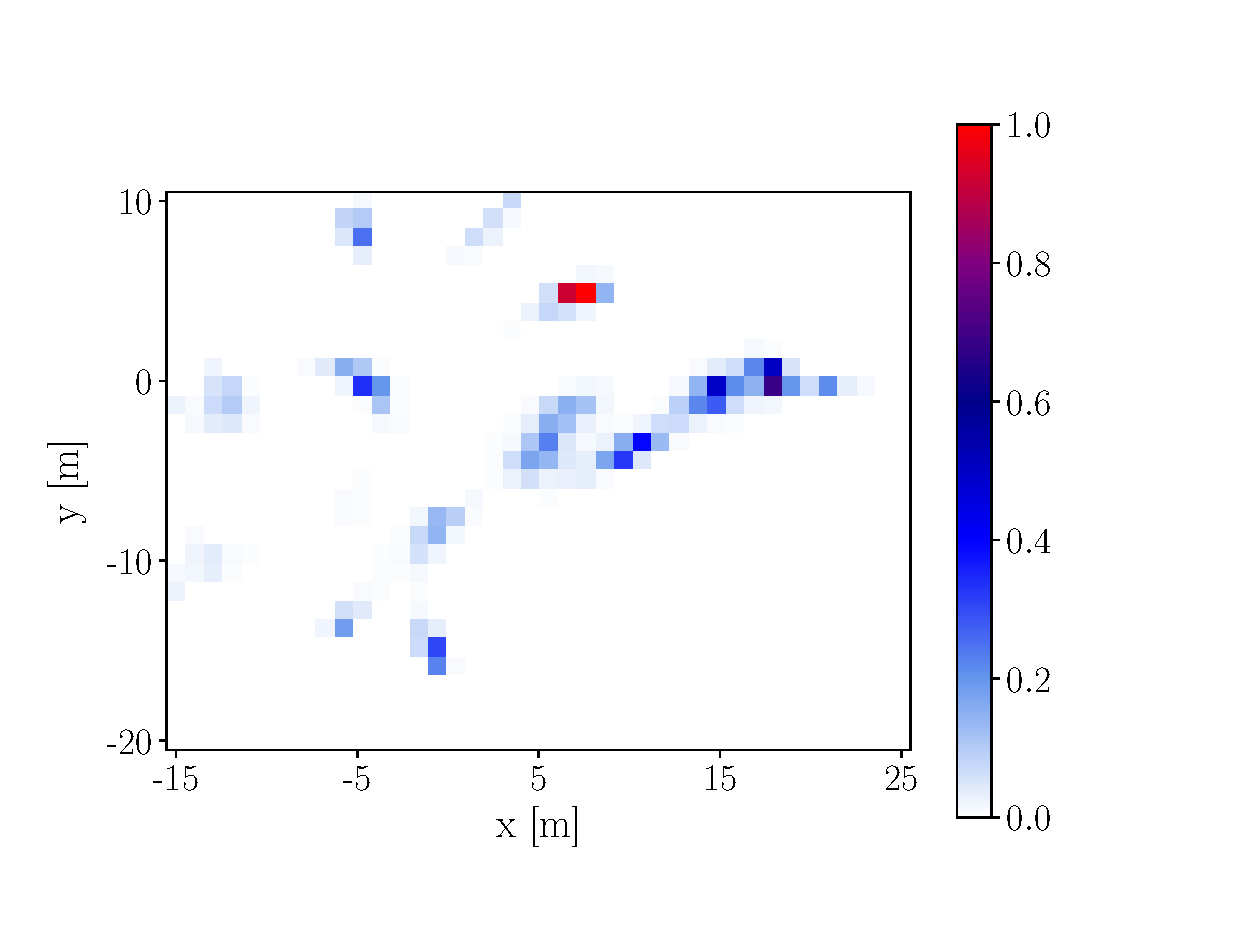
\includegraphics[width=0.5\textwidth,trim={0 0.5cm 2cm 1cm},clip]{./fig/photos/auto_simulation_lam_1.eps}
    \label{fig:}
  }
  \newline
  \noindent 
  \subfloat[sensitivity of detection $\mathbf{s}$] {
    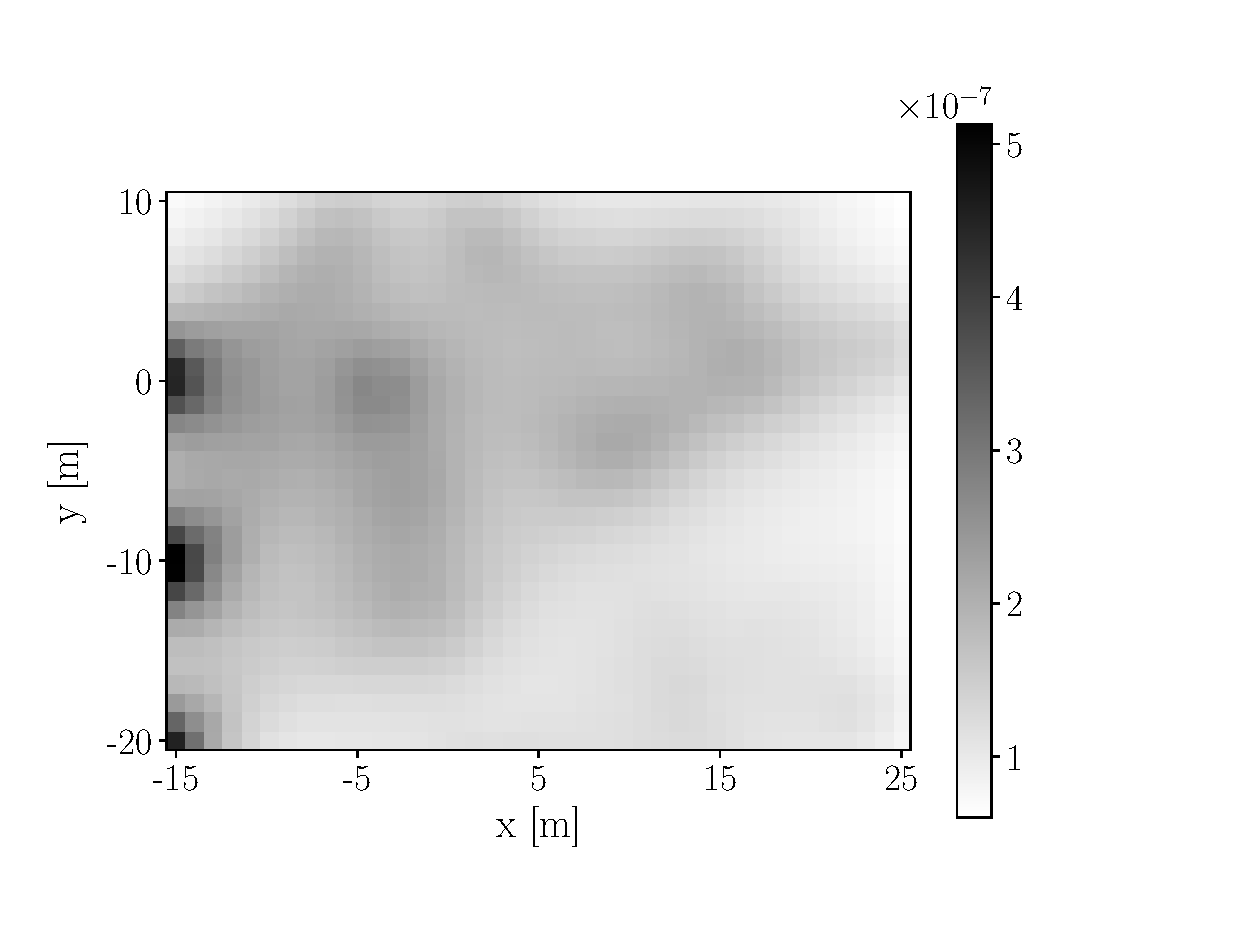
\includegraphics[width=0.5\textwidth,trim={0 0.5cm 2cm 1cm},clip]{./fig/photos/auto_simulation_sen_2.eps}
    \label{fig:}
  }
  \subfloat[sensitivity of detection $\mathbf{s}$] {
    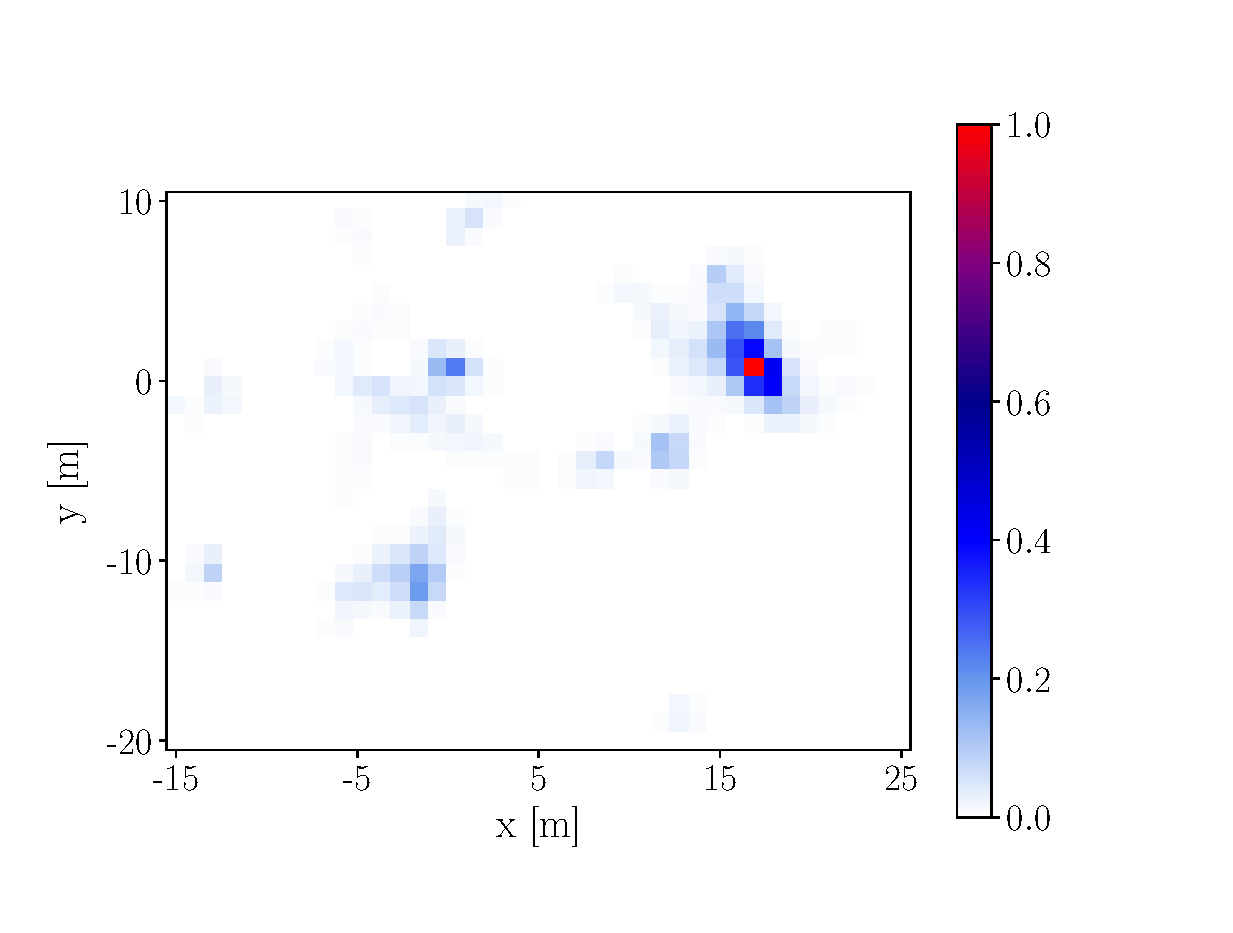
\includegraphics[width=0.5\textwidth,trim={0 0.5cm 2cm 1cm},clip]{./fig/photos/auto_simulation_lam_2.eps}
    \label{fig:}
  }
  %\subfloat[] {
  %  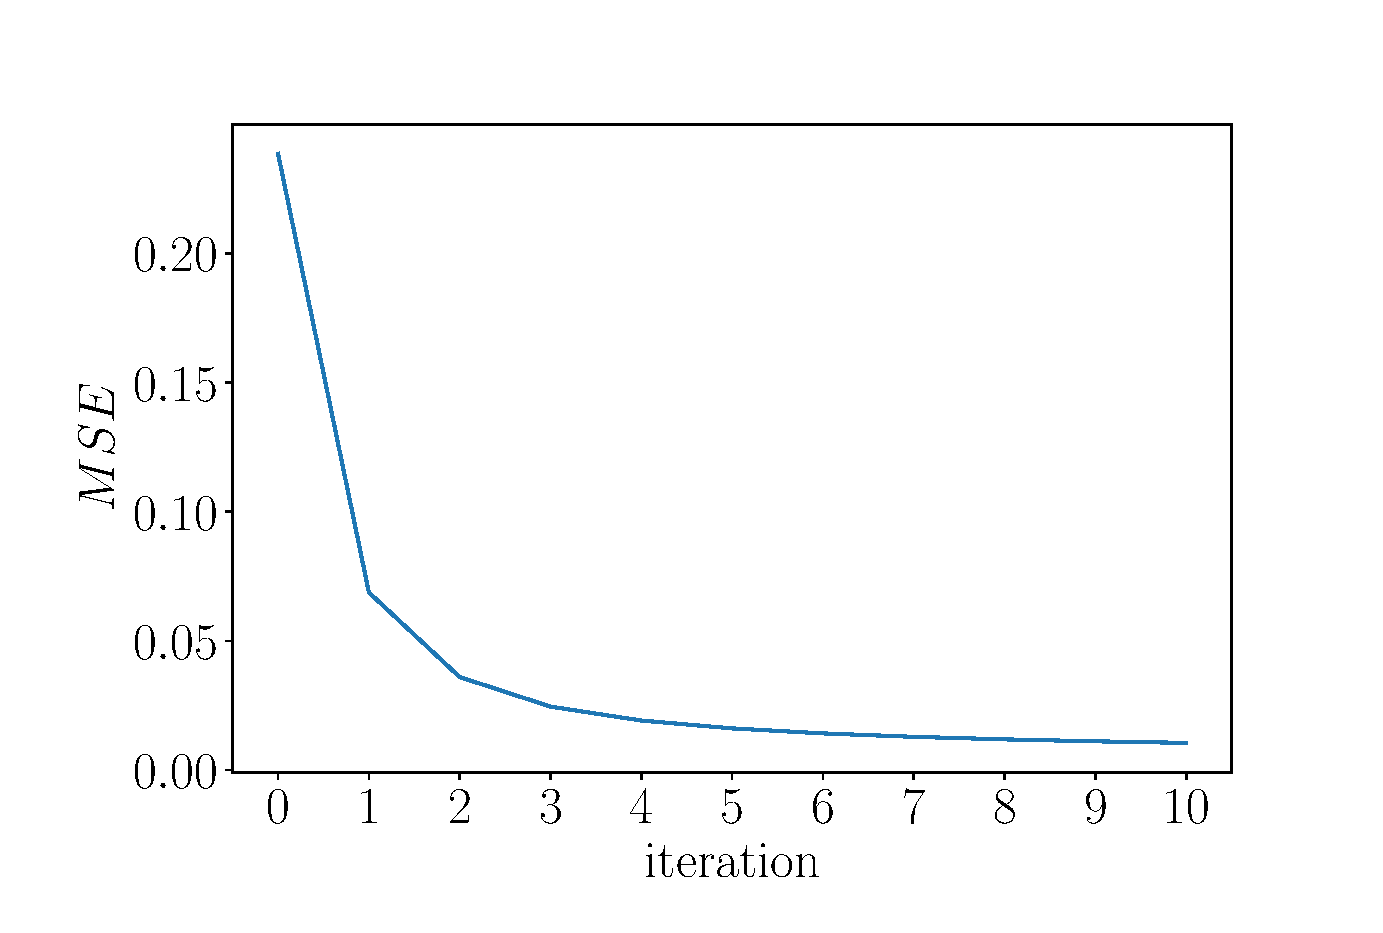
\includegraphics[width=0.5\textwidth,trim={0 0.5cm 2cm 1cm},clip]{./fig/photos/auto_mse_simulation.eps}
  %  \label{fig:}
  %}
  \caption{Results of Monte carlo simulation for cs137.Lorem ipsum  Lorem ipsum Lorem ipsum Lorem ipsum Lorem ipsum Lorem ipsum Lorem ipsum Lorem ipsum Lorem ipsum Lorem ipsum Lorem ipsum Lorem ipsum Lorem ipsum Lorem ipsum Lorem ipsum Lorem ipsum Lorem ipsum Lorem ipsum Lorem ipsum Lorem ipsum Lorem ipsum Lorem ipsum Lorem ipsum Lorem ipsum Lorem ipsum Lorem }
  \label{fig:e2}
\end{figure}% %%}

}% %%}
